\clearpage
\newpage
\section{Supplementary}
\subsection{Dataset Collection}\label{sup-datacollect}
This section introduces the collection of datasets used for the experiments conducted in this paper.

\subsubsection{Document Set Collection and Procession}
As no previous works focus on MD-QA, we create our own datasets to simulate real-world scenarios where users maintain folders containing various documents and pose questions to which the answers are only from certain parts of these documents. To imitate this scenario, we randomly sample questions from the development set of existing datasets: HotpotQA/IIRC/2WikiMQA/MuSiQue, and then for each specific question, we fetch documents from Wikipedia that encompass supporting facts pertaining to the question~\footnote{The HotpotQA/IIRC/2WikiMQA/Musique datasets already have the supporting facts for each question.} and term these documents as golden documents. Then we randomly sample negative documents from Wikipedia and pair them with golden documents to constitute the document collection. For each document in the collected document set, we split it into multiple passages with the default passage length being 250 as it empirically yields superior performance. As questions from these existing datasets only focus on document contents, we additionally incorporate the `PDFTriage' dataset, an internal company collection of real-world questions focusing on document structures. We refer readers to the paper~\cite{saad2023pdftriage} for more details.

\subsubsection{Knowledge Graph Construction}
We construct a knowledge graph for each question and its corresponding collection of documents. For datasets where the questions are from Wikipedia: HotpotQA, IIRC, WikiMHop, and Musique, we only have passage nodes since answering questions in these datasets does not require information about document structures. For the PDFTriage dataset, in addition to passage nodes, we apply ExtractAPI to obtain the page and table information so that the constructed KG also has pages/tables as nodes. For all of these datasets, we add edges following Section~\ref{sec-kgconstruct}. Table~\ref{tab-dataset} summarizes the average statistics of the document collections across all questions with their corresponding KGs. The code for the dataset collection and preprocessing is publically available at \url{https://github.com/YuWVandy/KG-LLM-MDQA}.

\begin{table}[htbp!]
\vspace{-2ex}
\scriptsize
\setlength\tabcolsep{2pt}
\caption{Statistics of document collections and their corresponding knowledge graph used in Table~\ref{tab-mainperform10} and \ref{tab-ablation} average across all questions.}
\centering
\begin{center}
\begin{tabular}{lcccccc}
\Xhline{2\arrayrulewidth}
\textbf{Dataset} & \#\textbf{Docs} & \#\textbf{Questions} & \#\textbf{Passages} & \#\textbf{Edges}& \textbf{\makecell{Passage \\Avg. Length}} & \textbf{\makecell{KG \\Density}} \\
\Xhline{2\arrayrulewidth}
HotpotQA & 12 & 500 & 715.22 & 70420.68 & 37.55 & 0.23\\
IIRC & 12 & 477 & 1120.55 & 143136.17 & 37.24 & 0.20\\
WikiMHop & 12  & 500 & 294.19 & 19235.15 & 37.24 & 0.27 \\
MuSiQue & 12 & 500 & 748.04 & 97931.28 & 38.56 & 0.29 \\
% Comp &  &  &  &  &  &  &  \\
\Xhline{2\arrayrulewidth}
\end{tabular}
\end{center}
\label{tab-dataset}
\vspace{-2ex}
\end{table}

More details about the PDFTriage dataset can be found at PDFTriage~\cite{saad2023pdftriage}.




\subsubsection{Sequential Data Collection} Training MDR~\cite{xiong2020answering} requires rearranging supporting facts into the sequential order that progressively approaches the answer. To fulfill this requirement, we directly follow MDR and use the pre-processed HotpotQA data from the GitHub Repository\footnote{https://github.com/facebookresearch/multihop\_dense\_retrieval/tree/main} to train the encoder and apply it to other datasets that do not provide the sequential order of supporting facts. For instruction fine-tuning LLaMA, we still use the above HotpotQA data and rearrange it into the instruction-input-output format and use the instruction `What evidence do we need to answer the question given the current evidence'. We present one example in Listing~\ref{list-InstructData}. For T5-large, we use the same input-output but prefix the reasoning instruction to the input following the original T5 input format~\cite{raffel2020exploring}.



\subsection{Experiment Details}\label{sup-exprdetail}
\subsubsection{Training DPR and MDR}
For training DPR~\cite{karpukhin2020dense}, we pair each question with its supporting facts as its positive passages, and some randomly sampled passages as its negative passages. For training MDR~\cite{xiong2020answering}, as each question in HotpotQA only requires 2 supporting facts to derive the answer, we set the first supporting fact as the positive pair for each question. Further, we concatenate this question and the first supporting fact to form a new question and for this newly-formed question, we set the second supporting fact as its positive pair. For both the original question and the concatenated one, we randomly sample other passages as the negative pair. Following~\cite{xiong2020answering, karpukhin2020dense}, we use RoBERTa-base as the default encoder. The search space of hyperparameters is summarized in Table~\ref{sup-tab-hyper-mdrdpr}.

\begin{table}[htbp!] 
\vspace{-1ex}
\footnotesize
\setlength{\extrarowheight}{0.5pt}
\setlength\tabcolsep{3pt}
\caption{Hyperparameters used for tuning DPR and MDR. The value of most of them are directly taken from their original GitHub Repository.}
\vspace{-2ex}
\label{sup-tab-hyper-mdrdpr}
\begin{center}
\begin{tabular}{m{13em} m{13em}}
\Xhline{2\arrayrulewidth}
\textbf{Hyperparameter} &  \textbf{Search Space}\\
\Xhline{2\arrayrulewidth}
Encoder & RoBERTa-base\\
Hidden Dimension & 768\\
Max Context Length & \{128, 256, 350\}\\
Batch Size & \{128, 256, 512\}\\
Epoch & 50\\
Warmup Steps & 300 \\
Learning Rate & 2e-5 \\
Gradient Clipping Range & 2 \\
\Xhline{2\arrayrulewidth}
\end{tabular}
\end{center}
\end{table}



\subsubsection{Instruction Fine-tuning LLaMA\footnote{\url{https://github.com/Lightning-AI/lit-llama}} and T5-Large\footnote{\url{https://shivanandroy.com/fine-tune-t5-transformer-with-pytorch/}}} We fine-tune LLaMA using instruction data in Listing~\ref{list-InstructData}. Due to the computational limitation, we choose LLaMA-7B and use LoRA~\cite{hu2021lora}. For fine-tuning T5-Large, we use the same instruction data except that we remove the instruction but only prefix the reasoning instruction to the input~\cite{raffel2020exploring}. We use the default hyperparameters from their original GitHub repository to fine-tune these two LLMs.


\subsubsection{Prompting LLMs for MD-QA - Table~\ref{tab-mainperform10} and \ref{tab-ablation}}
Following~\cite{trivedi2022interleaving}, we randomly select questions from the development set for reporting the performance. To ensure a fair comparison, we set the number of retrieved passages to 30 across all baselines and use ChatGPT as the downstream LLM for reading the retrieved passages and generating the answer. We summarize the key implementation details for each baseline as follows:
\begin{itemize}[leftmargin=*]
    \item \textbf{KNN}: We employ the sentence-transformer variant `multi-qa-MiniLM-L6-cos-v1' to obtain passage embeddings as it has been trained on 215M (question, answer) pairs from diverse sources. Then we select the top-15 passages according to the embedding similarity and the top-15 passages according to the fuzzy matching\footnote{We use Levenshtein-distance to measure the lexical distance between two passages.}.

    \item \textbf{MDR}: We use beam search with the inner product as the scoring function to rank passages. We limit the search depth to 2 as answering questions in HotpotQA requires at most 2-hop reasoning steps~\cite{xiong2020answering}. We set the number of passages to be 15 in the first-hop retrieval and for each of these passages, we further retrieve 3 more passages in the second round, which in total generates 45 passage pairs. Then we rank these 45 passage pairs by the product of the scores between the first-hop and the second-hop retrieval and select the top 30 ones as the final context.

    \item \textbf{IRCoT}: Instead of directly employing the original IRCoT code~\cite{trivedi2022interleaving}, we modify it based on our problem setting. The first reason is that passages to be retrieved in IRCoT~\cite{trivedi2022interleaving} are the pre-processed Wikipedia Corpus and do not cover the whole contents of Wikipedia documents, which thereby is not aligned with our MD-QA setting. The second reason is that the question-answering reader employed in IRCoT requires running on A100-80G GPU, which is not affordable on our side. Therefore, we modify the IRCoT by replacing the question reader with the ChatGPT and using our pre-processed Wikipedia document collections as introduced in Section~\ref{sup-datacollect}. For the prompt used in the reasoning step, we select 2 examples from `gold\_with\_2\_distractors\_context' for the demonstration purpose. We iteratively select top-5 passages based on the generated reason from LLM along with their document titles and add them to the retrieved context until hitting the prefix budget. For the prompt used in the reading step, we use exactly the same prompt as other baselines as we find it empirically leads to better performance than the original one used in IRCoT~\cite{trivedi2022interleaving}.

    \item \textbf{KGP-T5/LLaMA/MDR/ChatGPT}: We use T5-large/LLaMA-7B/MDR/ChatGPT as the LLM to guide the graph traversal respectively. For content-based questions, similar to MDR, we perform a 2-hop retrieval but for each hop, we only search the node to visit next from neighbor candidates. In the 1$^{\text{st}}$-hop retrieval, we select 10 passages and in 2$^{\text{nd}}$-hop retrieval, we select 3 passages, which totally forms 30 reasoning paths. Note that passages in the 1$^{\text{st}}$-hop retrieval are allowed to overlap with the ones in the 2$^{\text{nd}}$-hop retrieval. For structural-based questions, we first use ChatGPT to extract page/table structures and then fetch relevant contents in those structures. Future work could explore how to pre-train a structural extraction model to obtain document structures.

    \item \textbf{KGP-TF-IDF}: We remove the LLM-guided graph traversal but select passage nodes based on their TF-IDF similarity to the given question.

\end{itemize}

Note that we put the prompt template for running all the above baselines in Section~\ref{sec-prompt}.
 

\subsection{Complexity Analysis for KGP}\label{sup-KGP}

\SetAlCapSty{}
\SetAlgoNoEnd
\begin{algorithm}[htbp!]
 \DontPrintSemicolon
 \small
 \KwIn{A question $q$ over a set of documents $\mathcal{D}$, the constructed KG $G = \{\mathcal{V}, \mathcal{E}, \mathcal{X}\}$ over $\mathcal{D}$, the fine-tuned LLM-guided graph traversal $f_{\text{GT}}$, the preset context budget $K$, the TF-IDF search function $g$.}
 
Initialize seed passages $\mathcal{V}^s = g(\mathcal{V}, \mathcal{X}, q)$

Initialize the retrieved passage queue $\mathcal{P} = [\{v_i\}|v_i \in \mathcal{V}^{s}]$
 
Initialize the candidate neighbor queue $\mathcal{C} = [\mathcal{N}_i|v_i \in \mathcal{V}^s]$

Initialize the retrieved passage counter $k = \sum_{\mathcal{P}_i \in \mathcal{P}}|\mathcal{P}_i|$
 
\While{queue $\mathcal{P}$ and queue $\mathcal{C}$ are not empty}{
        $\mathcal{P}_i \leftarrow \mathcal{P}.\text{dequeue}()$, $\mathcal{C}_i \leftarrow \mathcal{C}.\text{dequeue}()$

        $\mathcal{V}_i' = \text{Graph Traversal}(\{q\}\cup \mathcal{P}_i, \mathcal{C}_i, k)$ by Eq~\eqref{eq-lmtraversal} 

        \For{$v \in \mathcal{V}_i'$}{
            $\mathcal{P}.\text{enqueue}(\mathcal{P}_i\cup \{v\})$, $\mathcal{C}.\text{enqueue}(\mathcal{N}_v)$

            $k \leftarrow k + 1$

            \If{$k > K$}{
                \textbf{Terminate}
            }
        }
    }
\KwRet{\text{Retrieved Passage Queue $\mathcal{P}$}}

\caption{\small LLM-based KG Traversal Algorithm to Retrieve Relevant Context for Content-based Question.}
% \label{alg-GPL}
\end{algorithm}


Since our algorithm can be essentially deemed as the combination of the neighborhood ranking by Eq.~\eqref{eq-lmtraversal} and the breadth-first-search. The time complexity would be the multiplication between the time of bread-first-search $\mathcal{O}(|\mathcal{V}| + |\mathcal{E}|)$ and the time of neighborhood ranking $\mathcal{O}(|\mathcal{N}|\gamma) = \mathcal{O}(\hat{d}\gamma)$ where $\gamma$ is the time for computing the embedding similarity between a specific neighbor passage and the retrieved reasoning path and $\hat{d}$ is the average degree of the KG. Therefore the final time complexity would be $\mathcal{O}((|\mathcal{V}| + |\mathcal{E}|)\hat{d}\gamma)$, which is in-between the linear and quadratic to the size of the graph. As users typically maintain 10-100 documents, correspondingly the number of nodes in the constructed KG would be around 1,000-10,000 (according to Table~\ref{tab-dataset}, a collection of 12 documents have roughly 200-1000 passage nodes), which is affordable even with the quadratic time complexity. Moreover, we can apply advanced techniques to further reduce the time complexity for neighborhood ranking, such as LSH~\cite{gionis1999similarity} and KD-tree~\cite{qu2020data}.


In addition, whenever there are some changes over the document set (e.g., the user adds a new document into the folder or removes an existing document), we can remove/add all sentence nodes from/to the graph. To guarantee the linear time complexity for removing sentences from one document, we need to maintain a pointer from the document to its sentence nodes. For adding sentence nodes of one document, we need to first apply the KG construction method to compute the lexical/semantic similarity between each of the newly added sentence nodes and the existing nodes in KG, and then add corresponding edges connecting them, which is also linear to the size of the current graph.

For space complexity, it takes $\mathcal{O}(|\mathcal{V}|(\alpha + \beta))$ to maintain the constructed KG on the fly where $\alpha$ is the average space for saving the passage embedding vector while $\beta$ is the average space for saving the textual information of that passage. Although our constructed KG treats passages as nodes, which cannot scale very well when the graph is extremely large, the total number of documents a user maintains in a folder is typically around 10-100, which is still affordable.



\subsection{Markdown-Formatted Table}\label{sup-KGP-table}
Figure~\ref{fig-tableunderstanding} demonstrates that by sending Tables in the markdown format, ChatGPT can successfully understand their content and perform information retrieval based on the given questions. However, we do observe that such a markdown-formatted solution is not feasible for the long table due to the input token limitation of ChatGPT, we plan to explore the solution using SQL as the prompt content or modeling the Table as the grid graph to solve the issue in the future.
\begin{figure}[htbp!]
    \centering
    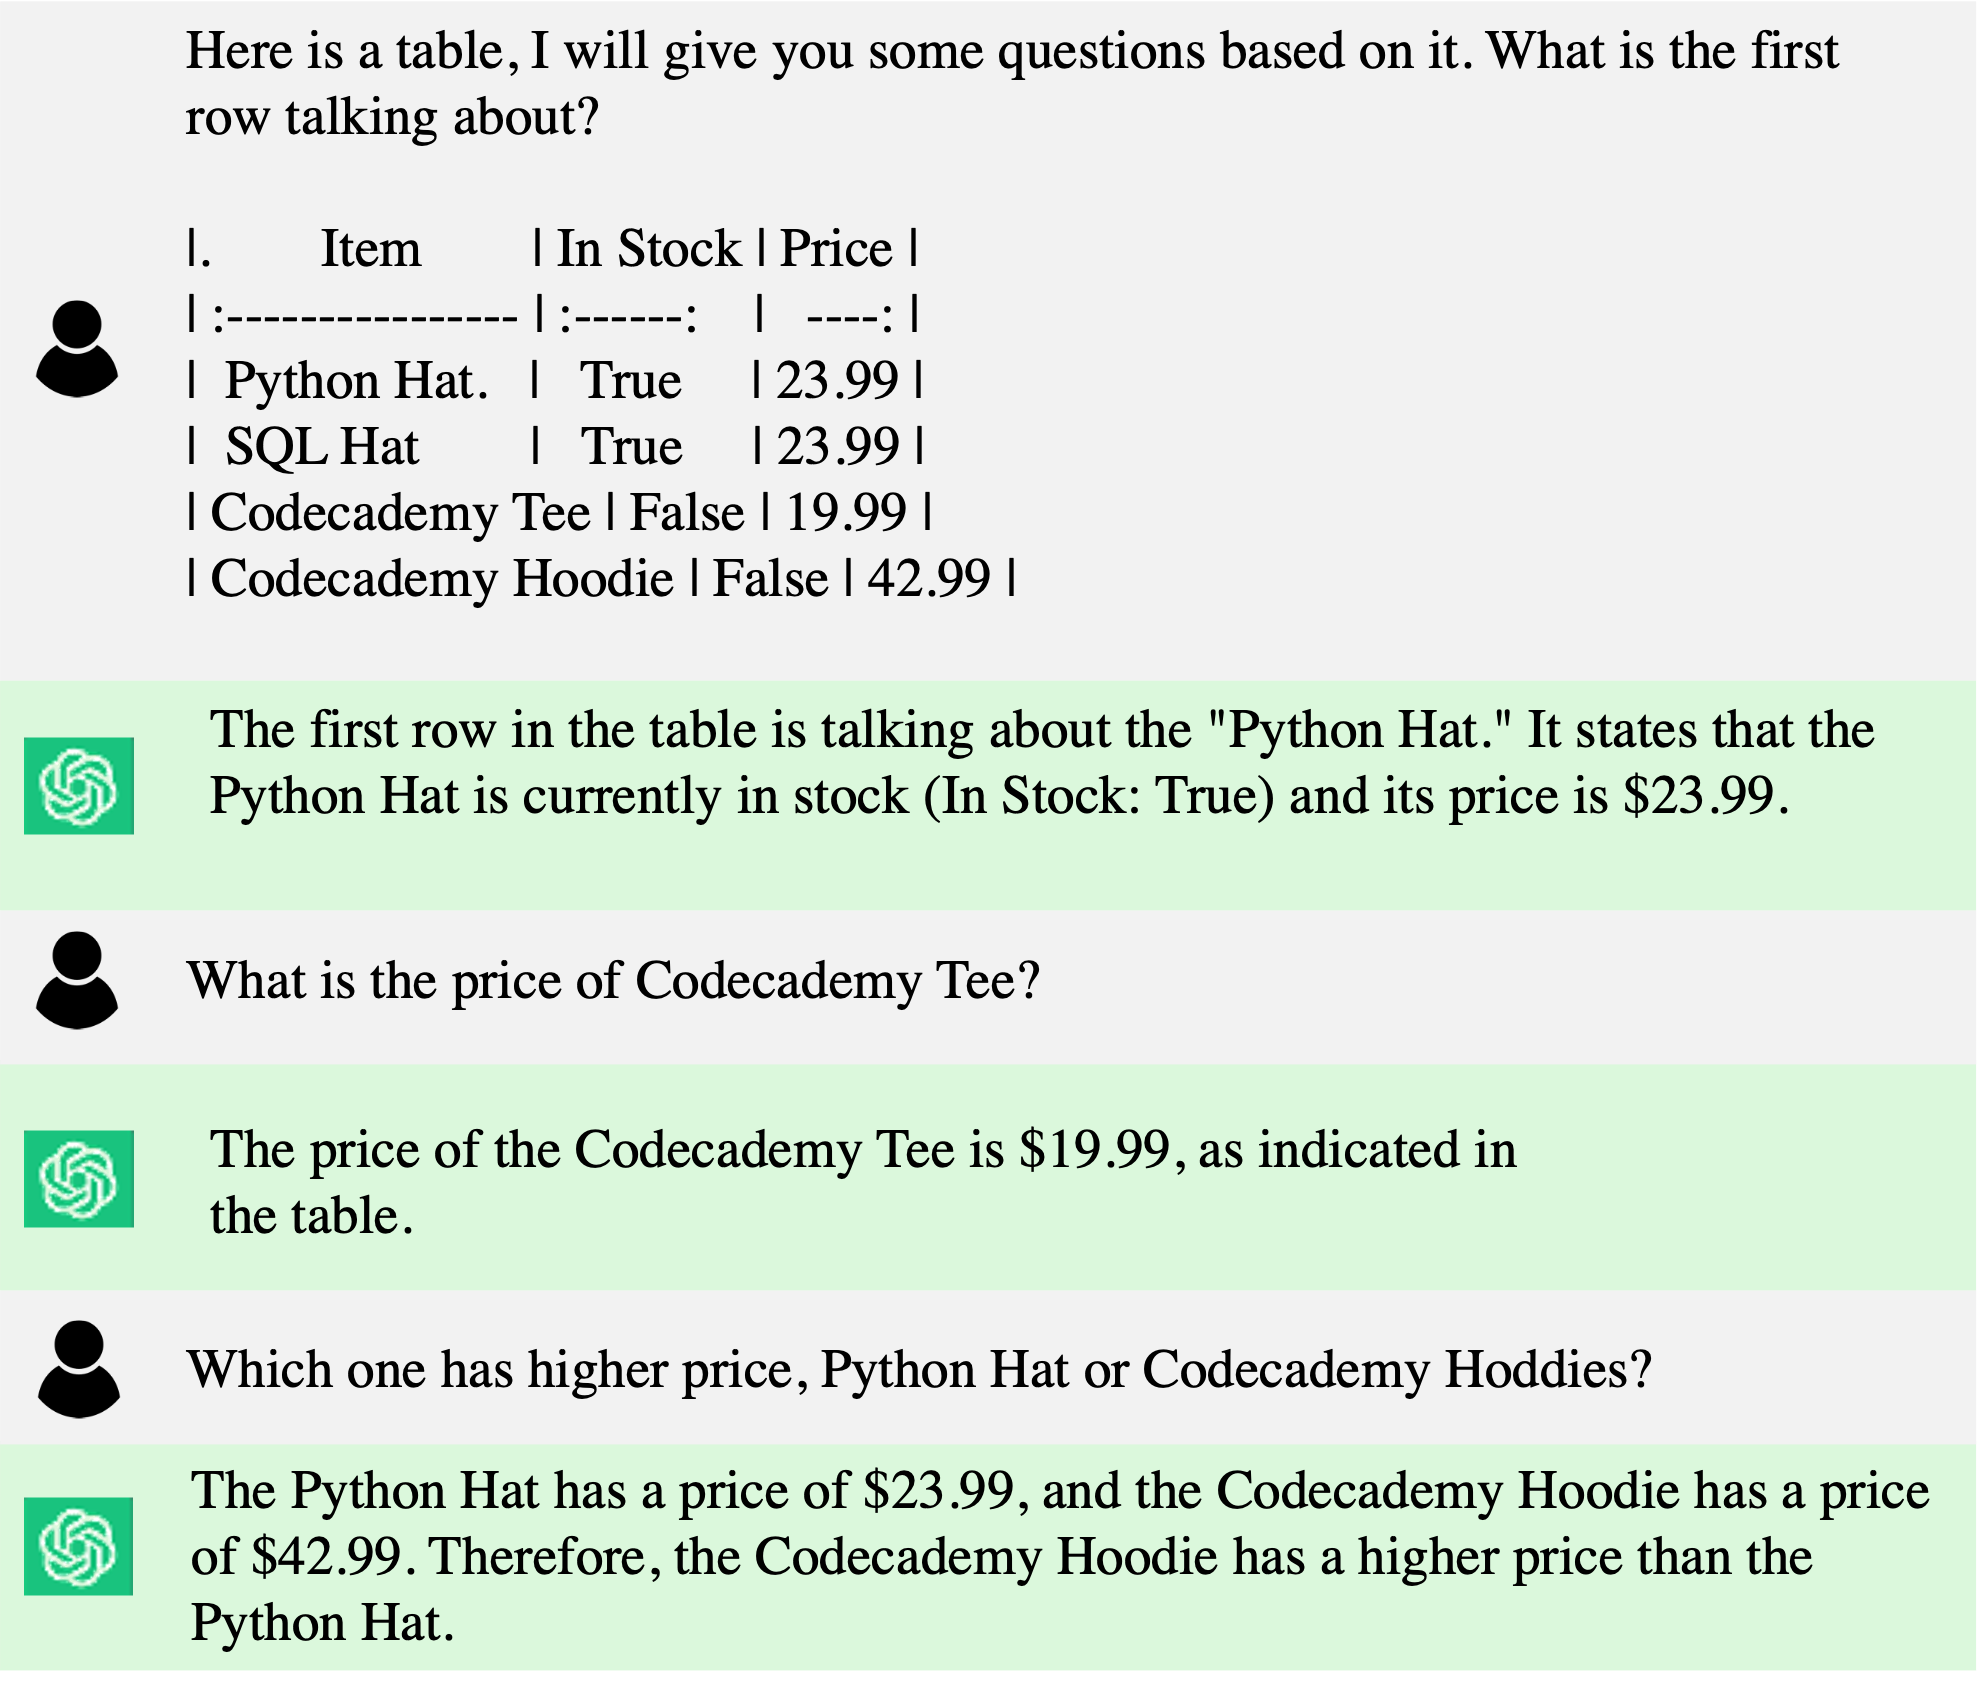
\includegraphics[width=0.48\textwidth]{Figure/tableunderstanding.png}
    \caption{An example demonstrating that ChatGPT can understand table in the markdown format.}
    \label{fig-tableunderstanding}
\end{figure}




\begin{table*}[t!]
\scriptsize
\setlength{\extrarowheight}{.095pt}
\setlength\tabcolsep{3pt}
\centering
\caption{Systematically Comparison among existing and our proposed Knowledge Graphs.}\label{tab-compare}
\begin{tabular}{lcccccc|c|c}
\hline
\textbf{KG} & \textbf{Node}& \textbf{Edge} & \textbf{Domain} & \textbf{Constructor} & \textbf{Scalability} & \textbf{Hyperparameters} & \textbf{Advantage} & \textbf{Disadvantage}\\
 \hline
\textbf{TAGME} & Passage & \makecell{Common \\Wikipedia Entity} & Wikipedia & / & No & Prior Threshold & \makecell{Effectively Identify \\Wikipedia Entities} & \makecell{Low efficiency for Entity Identification \\Narrow Domain Application} \\  
\hline
\textbf{TF-IDF} & Passage & Common Keyword & General & / & No & \# Keywords & No Domain Limitation & Common keywords irrelevant to question\\ 
\hline

\textbf{KNN-ST} & Passage & Semantic Similarity & General & \makecell{Sentence\\Transformer} & No & \# Neighbors & No Domain Limitation & Semantic Similarity irrelevant to question\\ 
\hline
\textbf{KNN-MDR} & Passage & Semantic Similarity & General & MDR & No & \# Neighbors & \makecell{Encoding the logical \\association for QA} & \makecell{Require logically ordered \\supporting facts to pre-train the model}\\  
\hline
\textbf{\makecell{Knowledge\\Base}} & Entity & Relationship & Specific & Human & Yes & / & \makecell{Powerful in encoding\\ factual information} & \makecell{Relation Extraction is non-trivial\\Domain Specific}\\  
\hline
\end{tabular}
\label{tab-kgconstruct}
\end{table*}

\subsection{Knowledge Graph Construction Comparison}\label{sup-KGC}
Table~\ref{tab-kgconstruct} compares different knowledge graph construction methods and their pros and cons. 

\begin{itemize}
    \item \textbf{TAGME}: TAGME~\cite{ferragina2010tagme} is very effective in extracting Wikipedia Entities from a passage despite the low efficiency. In our graph construction, it usually takes more than 8 hours to extract entities of all passages for even just 12 Wikipedia documents. Even after we apply parallel processing, it still takes more than 2 hours. In addition, it can only handle entities mentioned in the existing Wikipedia system and hence cannot generalize to documents from other domains. 

    \item \textbf{TF-IDF and KNN-ST}: Although there is no domain limitation, it is hard to guarantee the extracted keywords or the embedding semantic similarity can precisely encode the relationships that are desired for answering the given question between any two passages. We empirically find TF-IDF is more likely to extract meaningless keywords even after removing supporting verbs and articles.

    \item \textbf{KNN-MDR}: Since KNN-MDR pre-trains the sentence encoder by predicting the next supporting passage given already-retrieved passages, the embedding similarity between two passages is more likely to encode necessary logical associations required for MD-QA. However, the main bottleneck here is how to obtain the logically ordered supporting facts that can progressively reach the answer. Obtaining these sequential data is non-trivial and usually requires a large number of human resources for well-curated annotation.

    \item \textbf{Existing Knowledge Base}: One common approach in the literature is to use existing knowledge bases or extract subgraphs from them for specific tasks~\cite{yasunaga2022deep, dong2023hierarchy, yasunaga2021qa}. Because the factual information is characterized as a triplet consisting of two entity nodes and their relationship, it is very powerful in encoding factual information/commonsense knowledge and also avoids the scalability issue (since two different passages might share the same entity). Despite its potency and ease of use, constructing this type of KGs demands meticulously designed relation extractors, which is still deemed a challenging task in the literature. Recent research has explored using LLMs for relation extraction. However, with increasing document numbers, using non-open-sourced LLMs can become prohibitively expensive. A potential solution is fine-tuning an open-sourced LLM specifically for relation extraction. Detailed discussion on this is beyond the scope of this study and is thus omitted.
\end{itemize}

To put it in a nutshell, there's no one-size-fits-all method for KG construction. Our paper offers an in-depth analysis of the proposed KG construction methods alongside other existing ones. The best approach often depends on the specific use case. For broad domains containing general factual information, tools like 'TAGME' or 'Knowledge Base' might be apt. However, for more niche or sensitive areas, methods like TF-IDF/KNN-ST are more appropriate. In certain situations, gathering domain-specific data and pre-training encoders is the most effective way to build the KG.


\newpage
\subsection{Additional Results and Discussions}\label{sup-res}
\subsubsection{Quality of KG on MuSiQue}
Similar to the setting used for Figure~\ref{fig-hotpotqa_graph}, we change the hyperparameters to construct KGs for each question in MuSiQue with varying levels of sparsity and measure how much percentage of the supporting facts are covered by neighbors of the seeding passages that are initially retrieved by TF-IDF. The general trend is similar to the one in Figure~\ref{fig-hotpotqa_graph}, i.e., as the graph becomes denser, the precision decreases while the SF-EM increases. However, on MuSiQue, KNN-MDR achieves the worst trade-off between Precision and SF-EM compared with KNN-ST and TF-IDF. This is because our KNN-MDR is pre-trained on HotpotQA and due to the distribution shift from HotpotQA to MuSiQue, it is expected for the graph constructed with KNN-MDR to have less quality. Note that although here KNN-ST leads to a better KG than KNN-MDR, it does not mean the KNN baseline in Table~\ref{tab-mainperform10} should perform better than MDR because the baseline name only refers to the retrieval method while the name in this figure refers to the KG construction method.

\begin{figure}[htbp!]
    \centering
    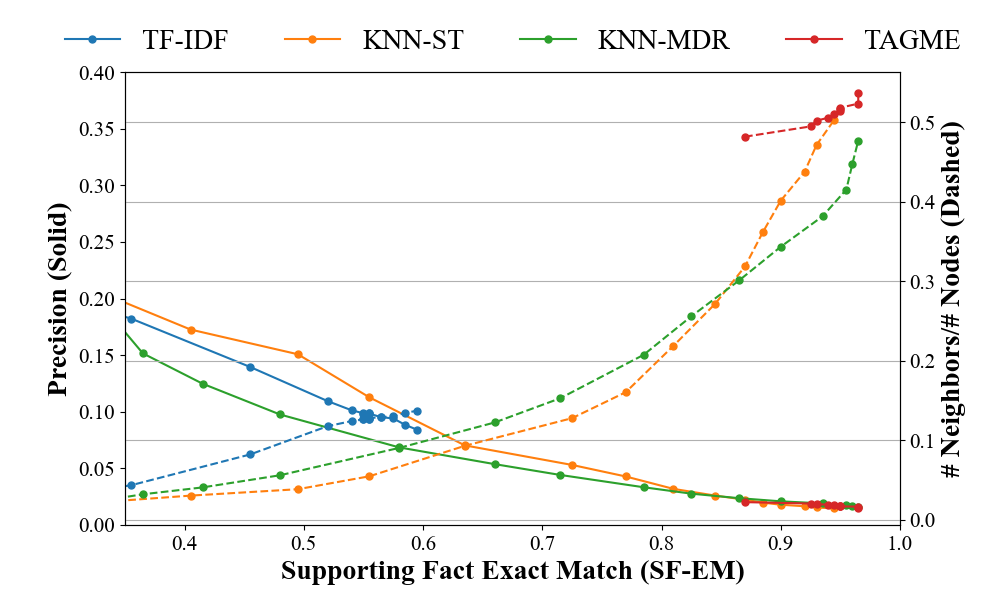
\includegraphics[width=0.48\textwidth]{Figure/musique_graph.png}
    \caption{Quality of constructed KGs with different methods on MuSiQue. \textbf{TF-IDF}: lexical similarity based on common keywords extracted by TF-IDF. \textbf{KNN-ST}: KNN graph constructed based semantic similarity of embeddings from sentence-transformer; \textbf{KNN-MDR}: KNN graph constructed based on semantic similarity of embeddings from the pre-trained MDR~\cite{xiong2020answering}; \textbf{TAGME}: graph constructed based on whether two passages share common Wikipedia entity mentions}
    \label{fig-musique_graph}
\end{figure}


\subsubsection{The impact of KG on MuSiQue}
Similar to the setting used for Figure~\ref{fig-hotpotqa_graph_perform}, we compare the MD-QA performance for KGP-T5 using TAGME-based KG with different levels of density. Similar to Figure~\ref{fig-hotpotqa_graph_perform}, here we also observe that as the KG becomes denser, the MD-QA performance increases while the time for the next node search increases. However, on MuSiQue, in most cases, KNN-ST achieves better F1/EM than KNN-MDR, which exactly aligns with the constructed KG quality observed in Figure~\ref{fig-musique_graph}, i.e., KNN-ST achieves better Precision/SF-EM trade-off than KNN-MDR on MuSiQue.


\begin{figure}[t!]
    \centering
    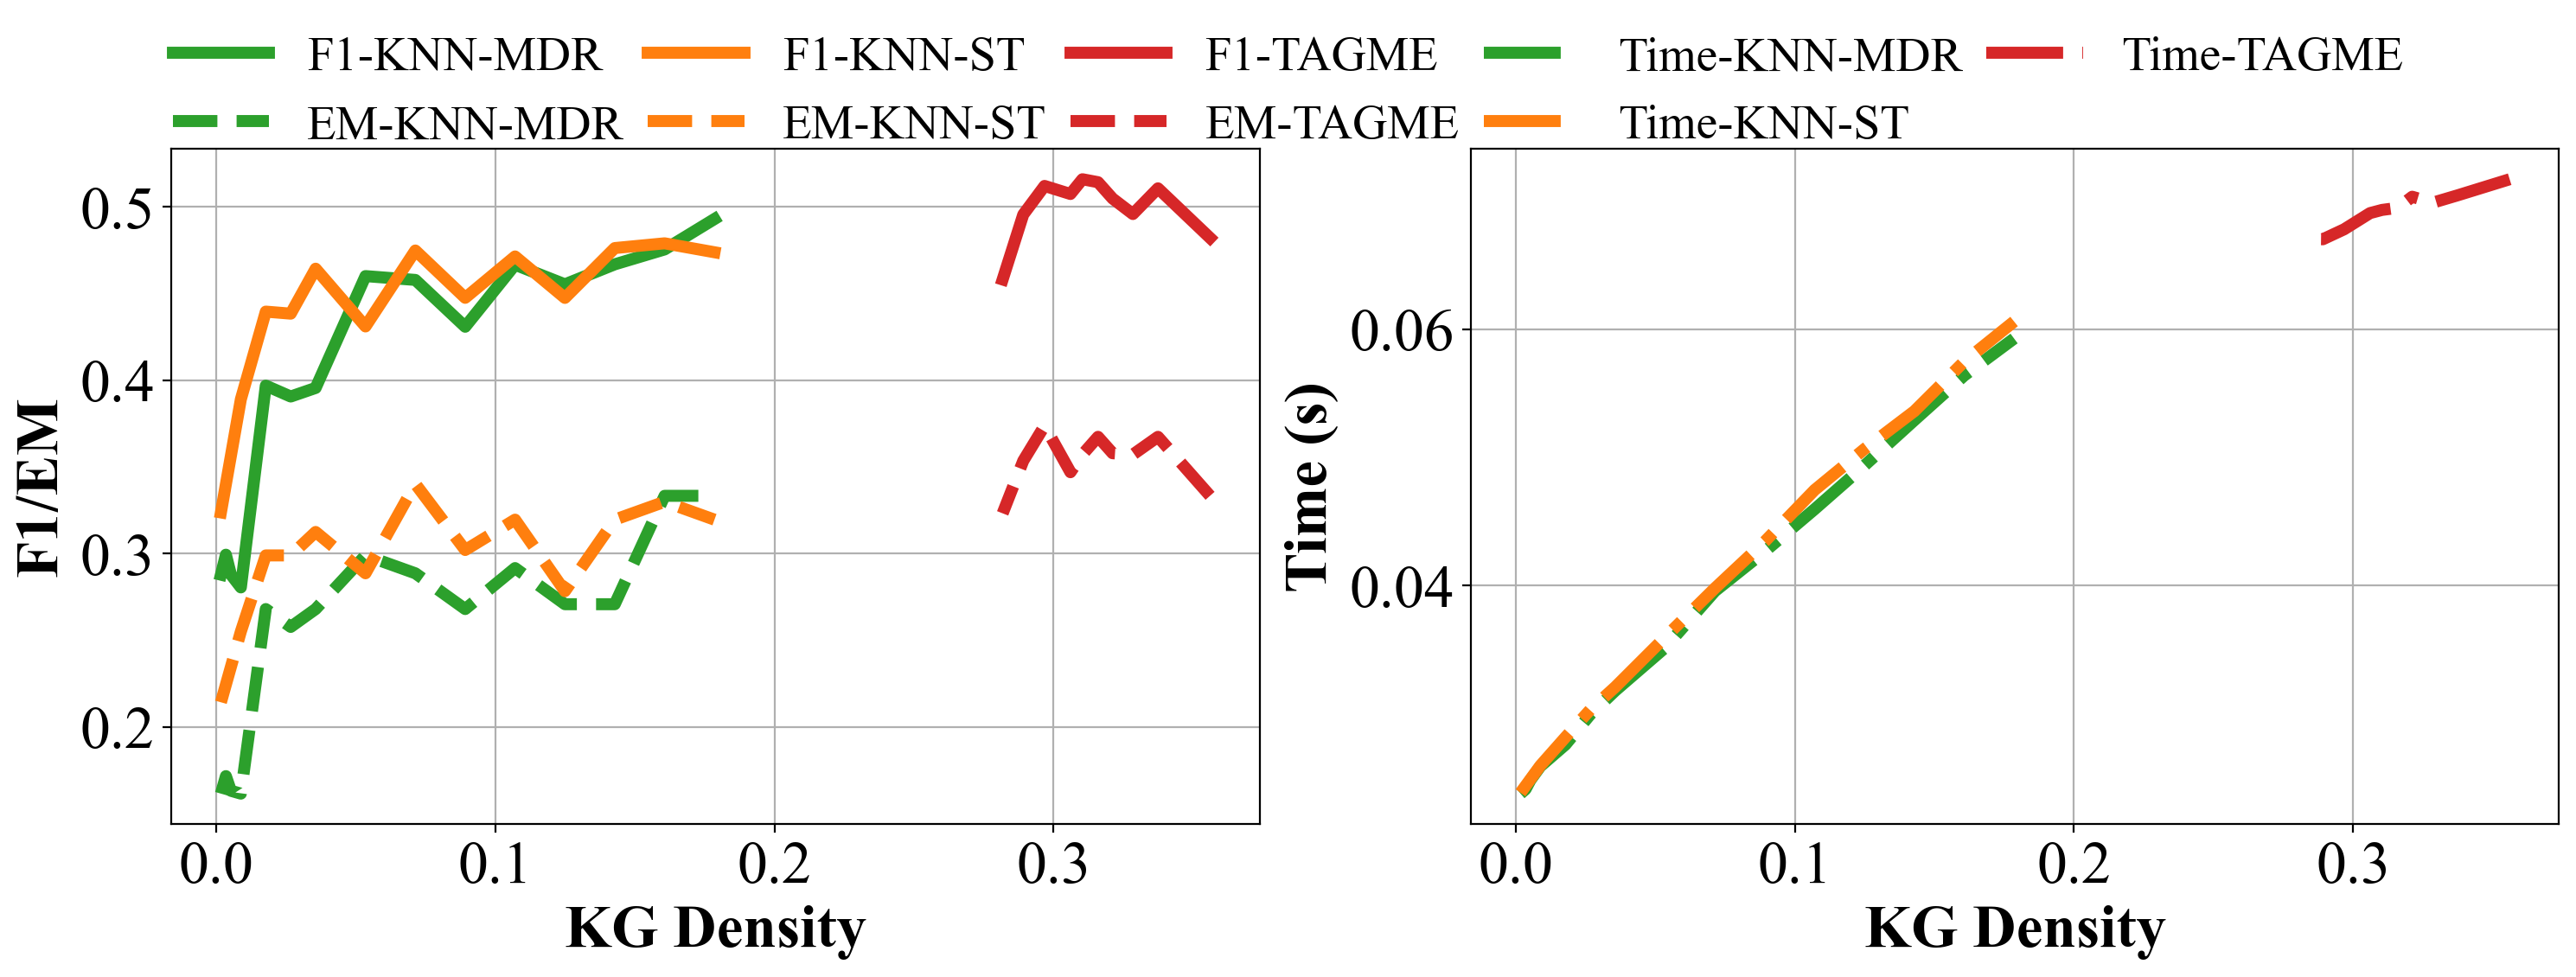
\includegraphics[width=0.48\textwidth]{Figure/combined_graph_musique.png}
    \caption{The performance/latency increases as the KG density increases. The results are averaged across 100 randomly sampled questions on MuSiQue.}
    \label{fig-musique_graph_perform}
\end{figure}

\subsection{Case study on Structural/Content Questions}\label{sec-casestudy}
In this section, we conduct six MD-QA case studies using our self-designed user interface coupled with the proposed method on the backend. Examples include two table-based QA (Figure~\ref{fig-Table1-ex}-\ref{fig-Table2-ex}), one page-based QA (Figure~\ref{fig-Page-ex}), one single-document content-based QA (Figure~\ref{fig-singledoc-ex}) and two multi-document content-based QA (Figure~\ref{fig-LBJOhio-ex1}-\ref{fig-MJLBJ-ex2}). In our designed interface, we can upload documents we are interested in reading and the model on the backend will split each of them into multiple passages. In addition, on the left side, we can ask questions related to the currently uploaded documents. By clicking the button `SUBMIT', the question would be sent to the model on the backend and it retrieves relevant context and arranges them as the prompt to get the answer from ChatGPT. In the figures below, we can see our system can understand the Table/Page questions and also questions requiring knowledge across multiple documents.


\onecolumn


\begin{figure}[htbp!]
    \centering
    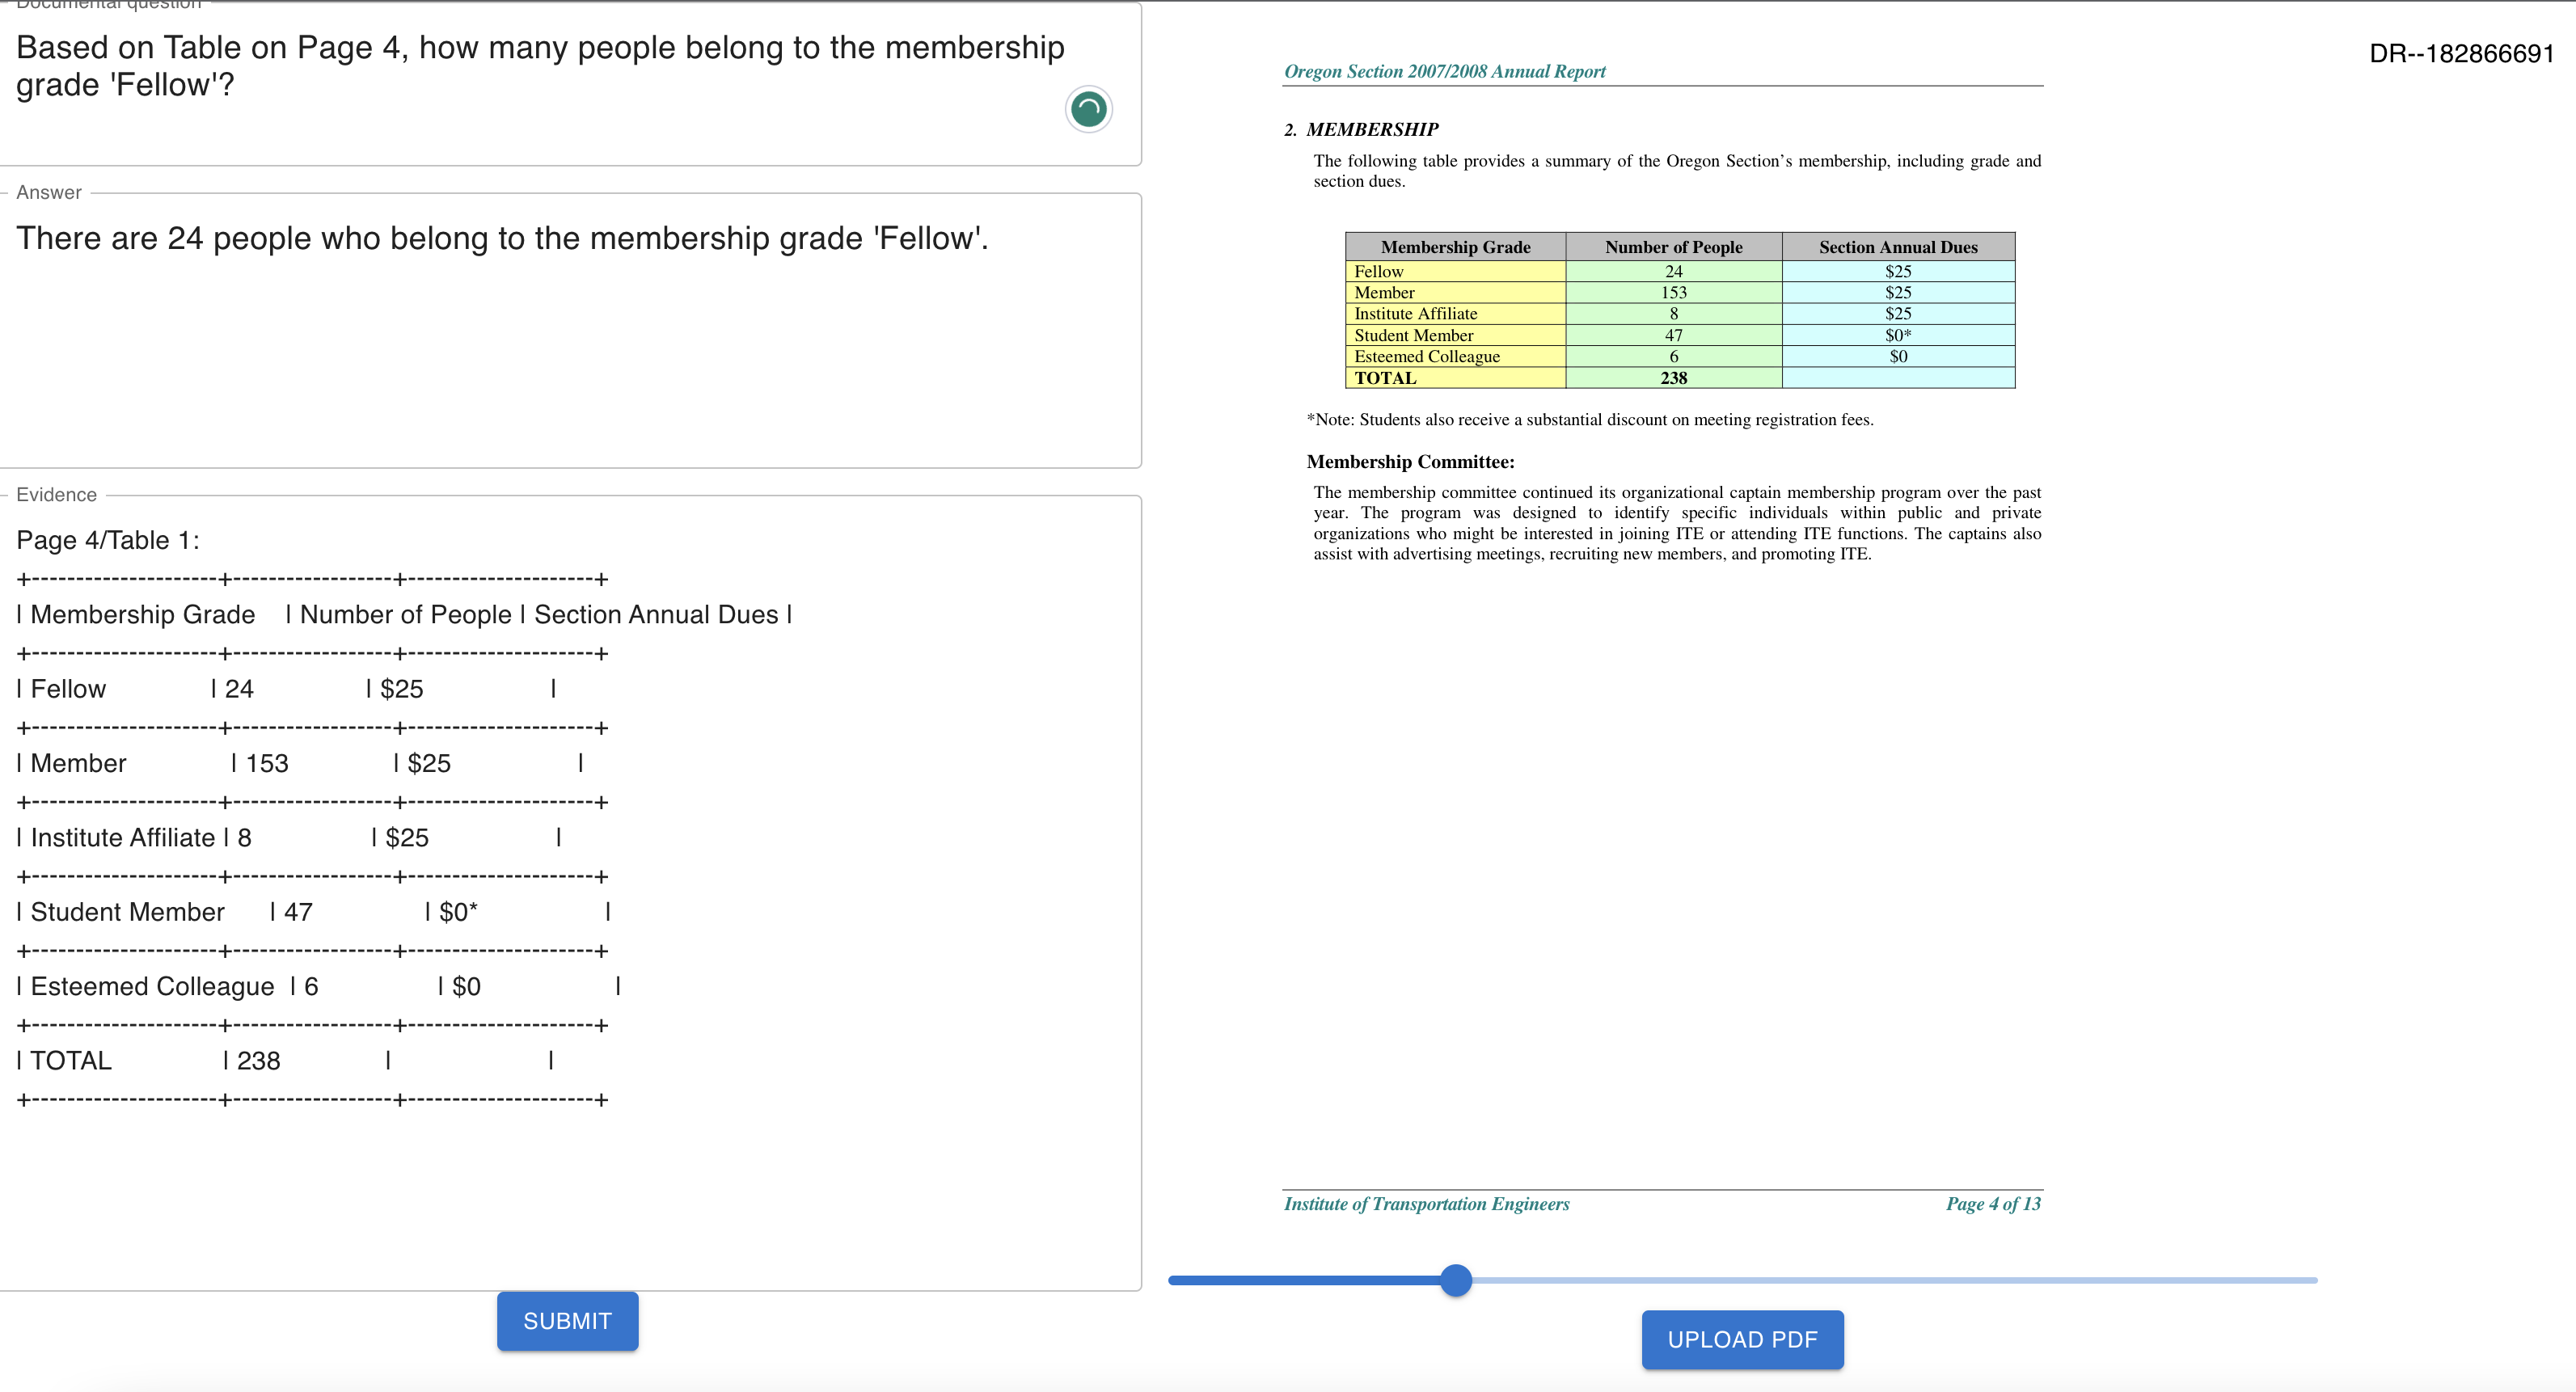
\includegraphics[width=\textwidth]{Figure/Table1-ex.png}
    \caption{Table QA asking for the number of people belonging to the membership grade `Fellow'. It is shown that ChatGPT can understand table structure in the format of markdown and successfully fetch the number of people belonging to membership `Fellow'.}
    \label{fig-Table1-ex}
\end{figure}

\begin{figure}[htbp!]
    \centering
    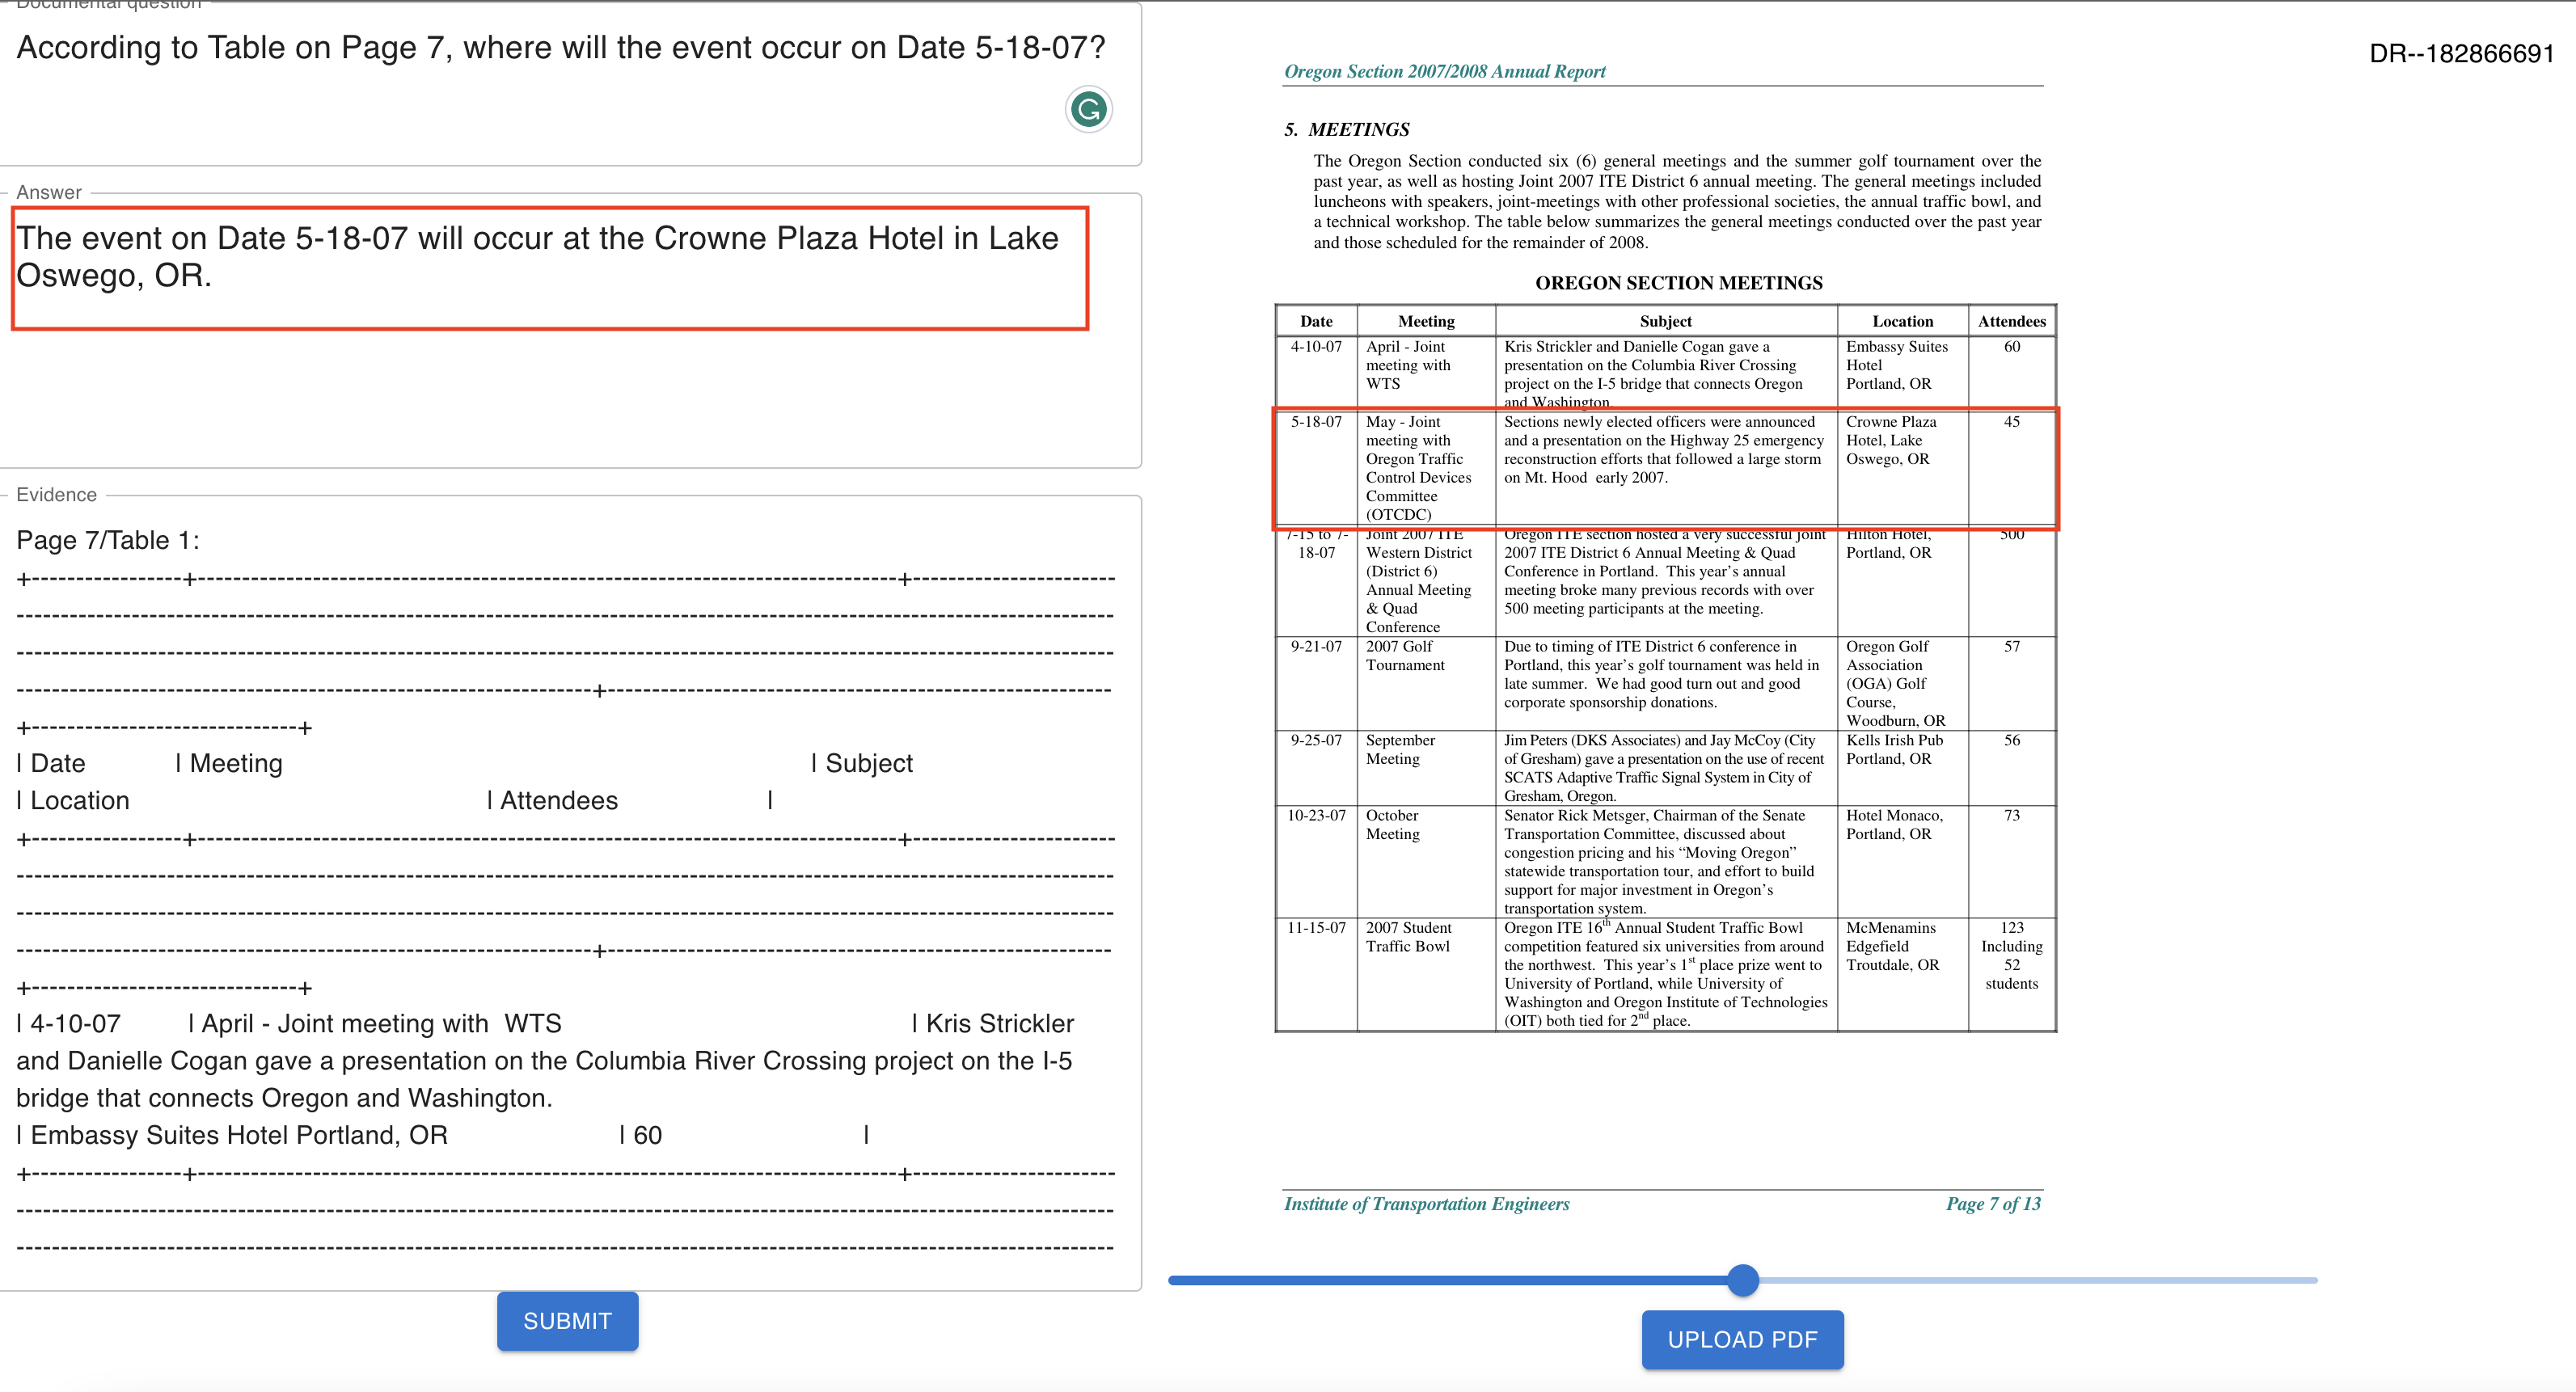
\includegraphics[width=\textwidth]{Figure/Table2-ex.png}
    \caption{Table QA asking for the place where the event on Date 5-18-07 will occur.}
    \label{fig-Table2-ex}
\end{figure}

\begin{figure}[htbp!]
    \centering
    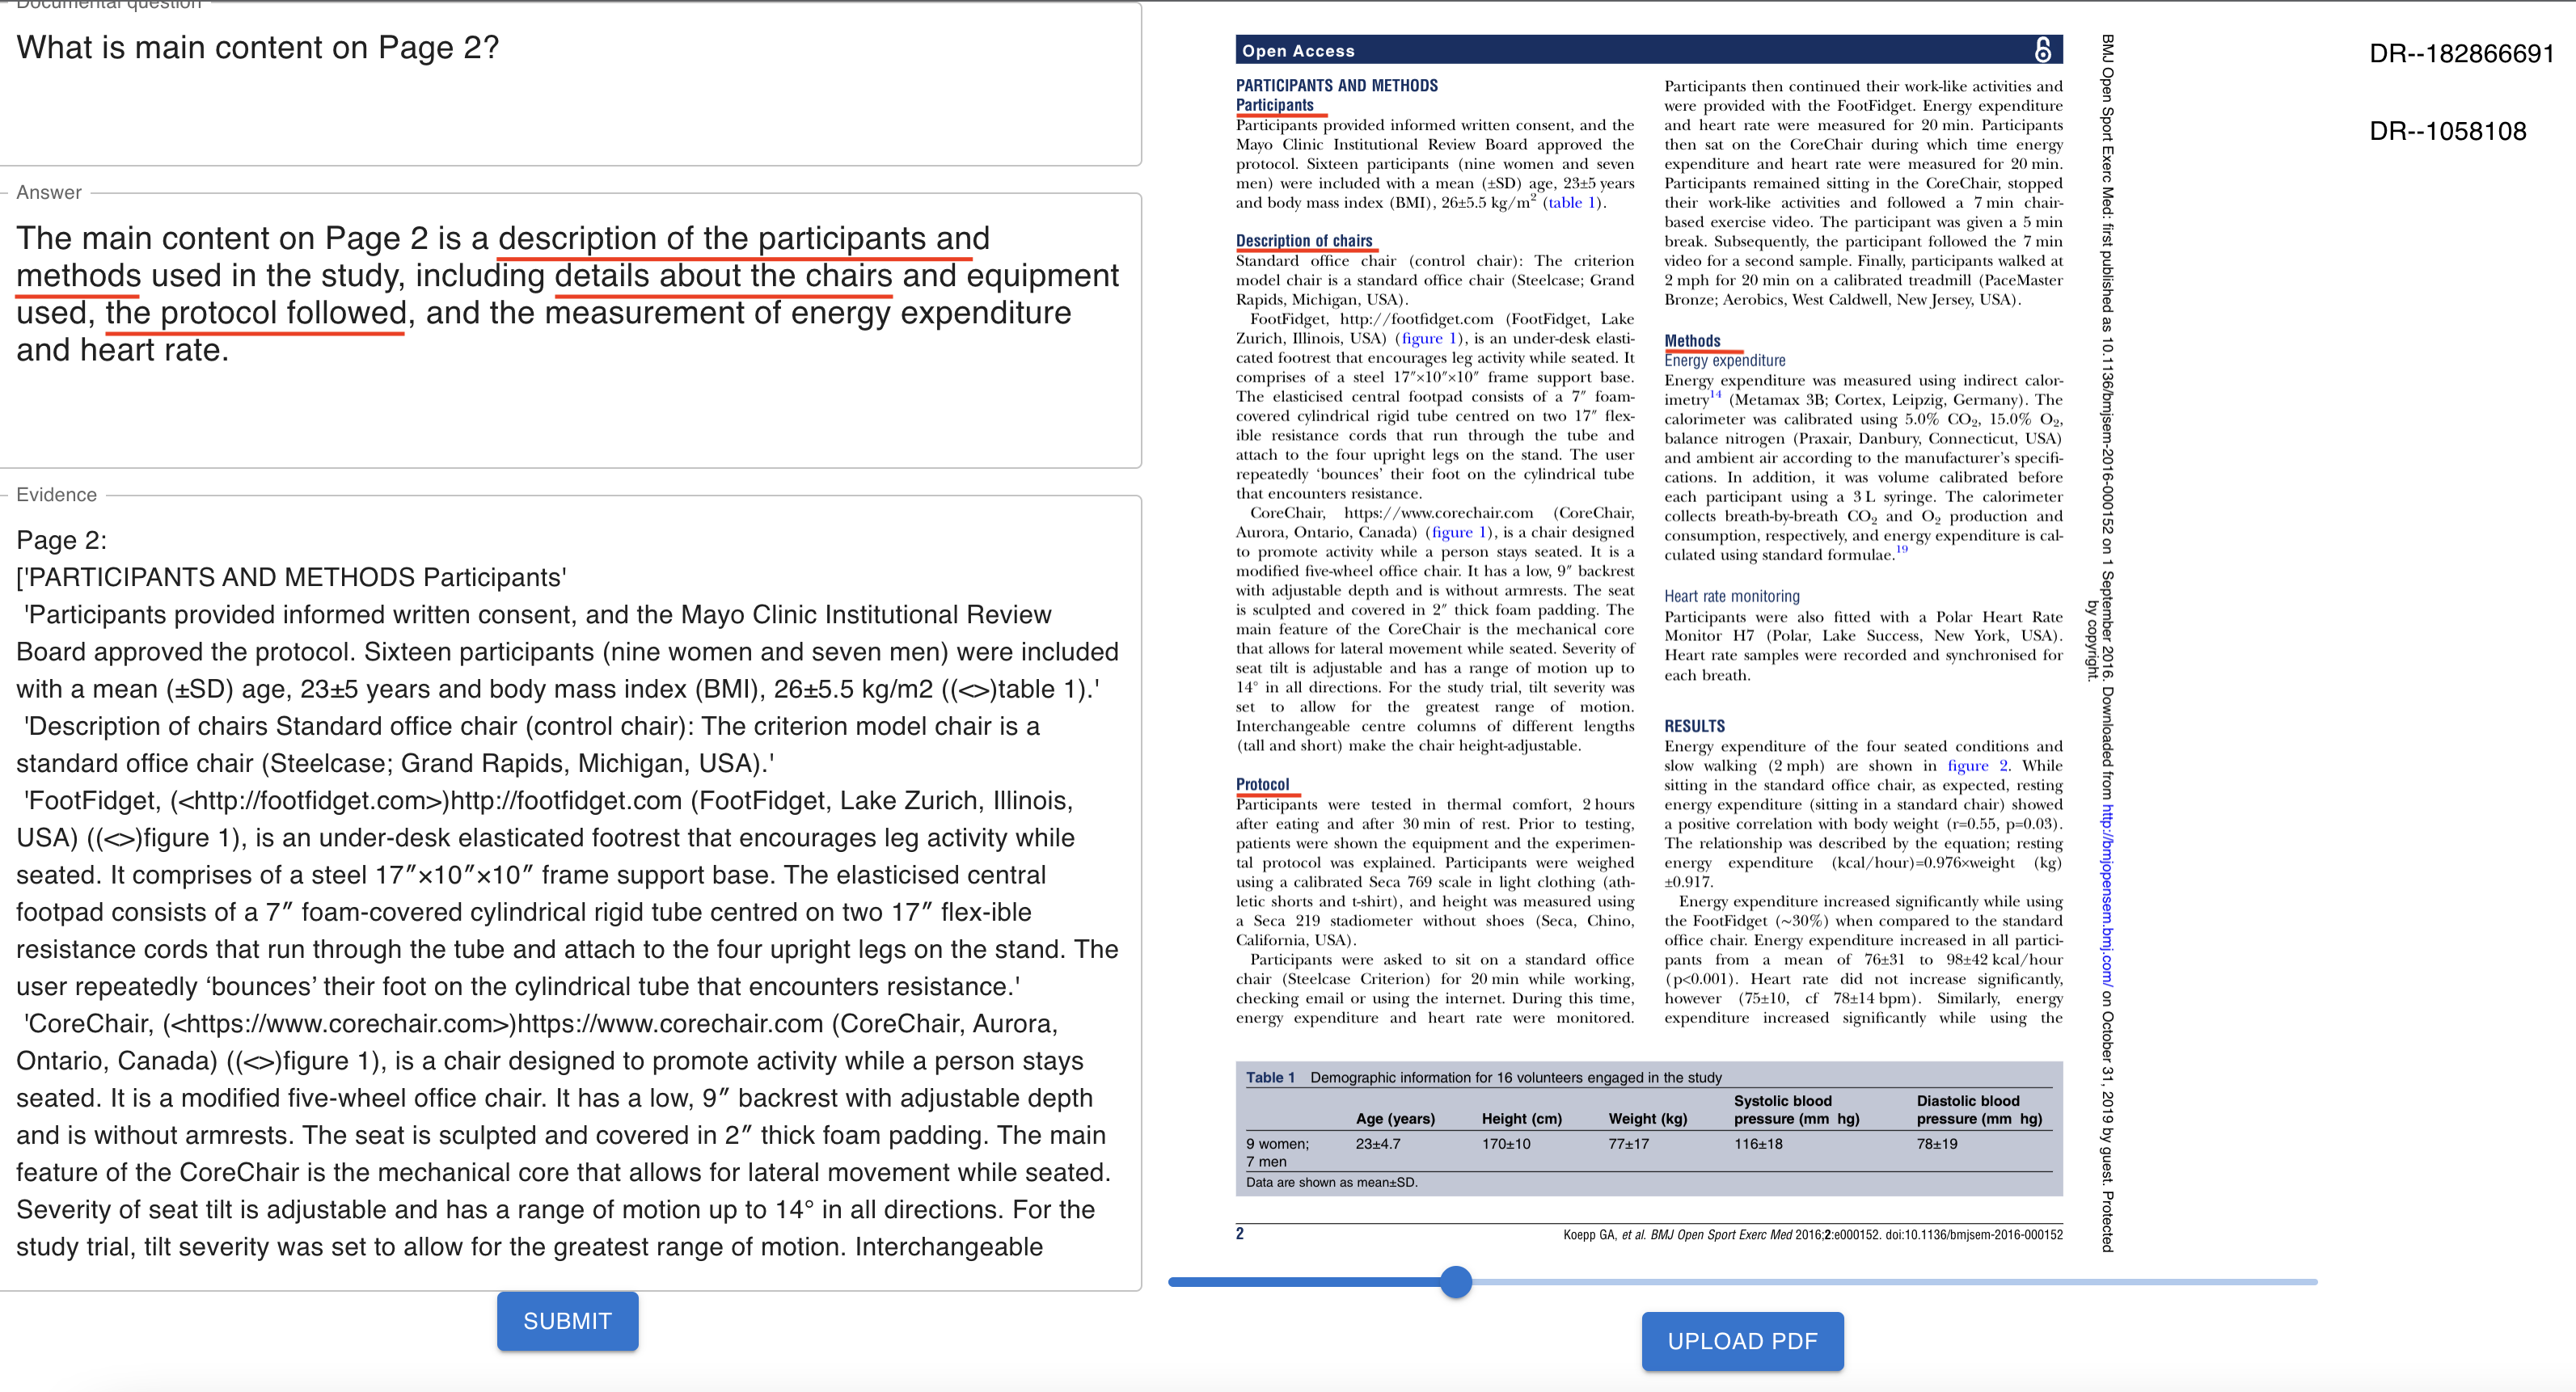
\includegraphics[width=\textwidth]{Figure/Page-ex.png}
    \caption{Page QA asking the main content on Page 2. The answer provides a high-level summarization of Page 2, covering the title of each section.}
    \label{fig-Page-ex}
\end{figure}

\begin{figure}[htbp!]
    \centering
    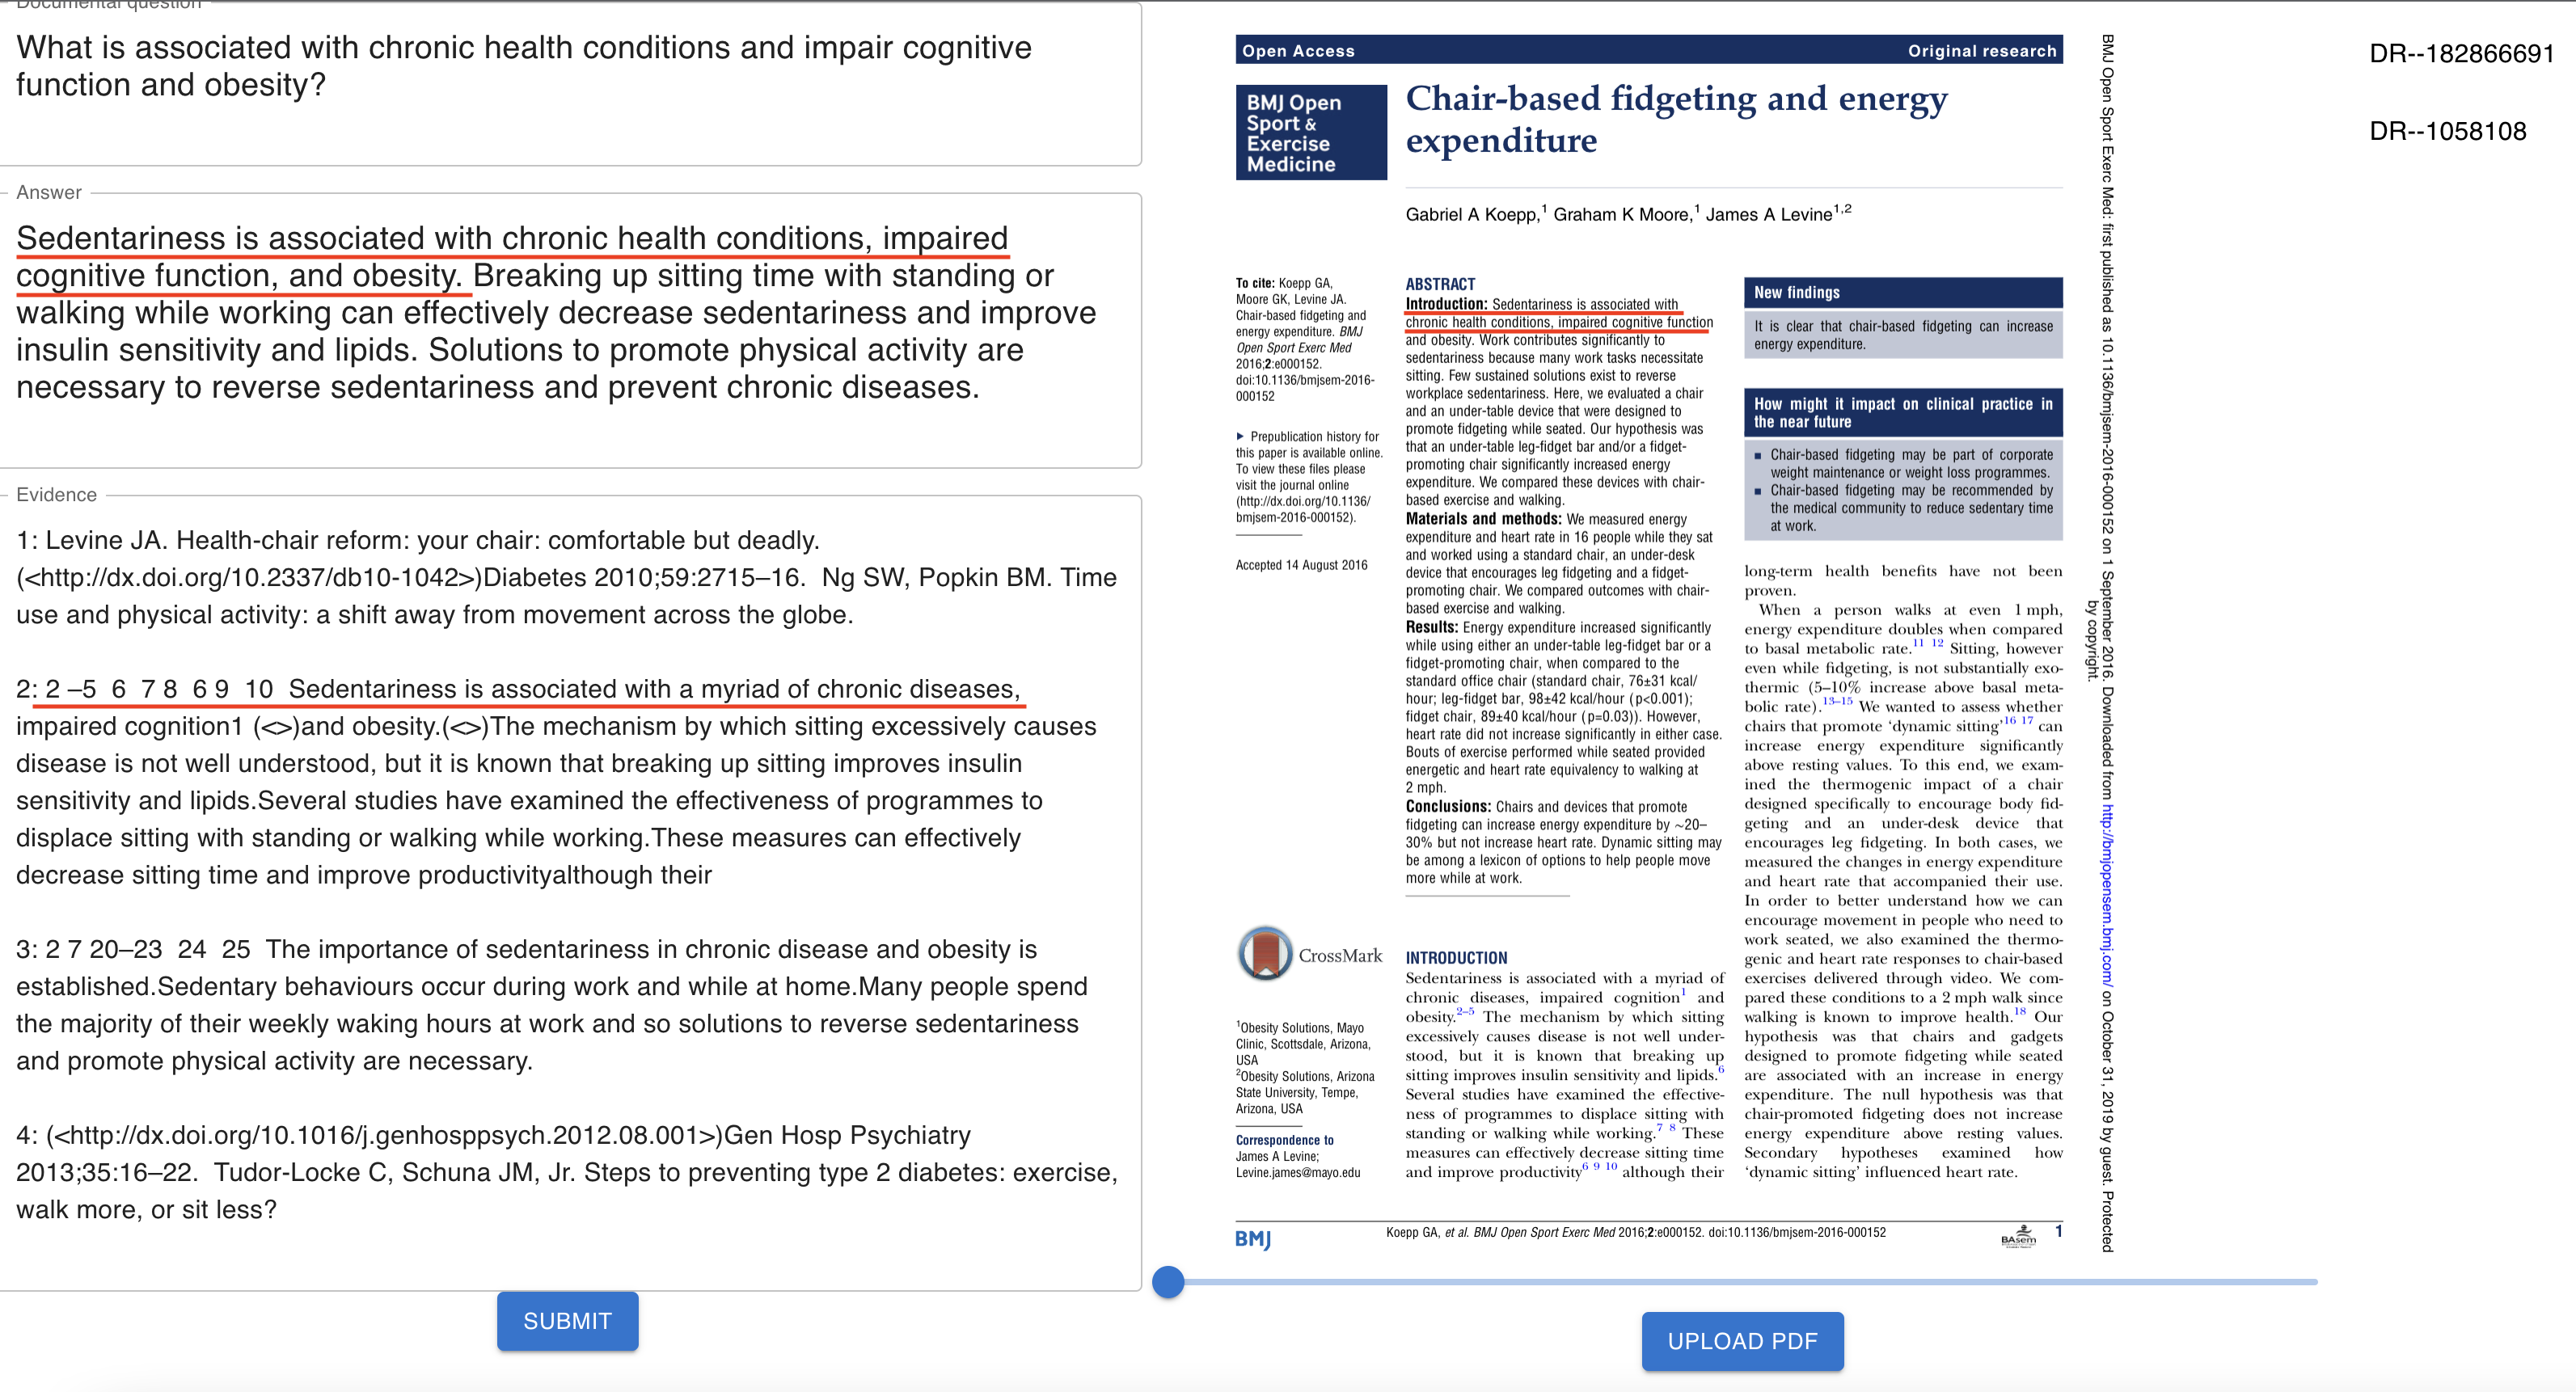
\includegraphics[width=\textwidth]{Figure/Singledoc-ex.png}
    \caption{Single Document Content QA asking Sedentariness. The 2$^{\textbf{nd}}$ retrieved sentence includes the answer and corresponds to the first sentence in the abstract of the paper.}
    \label{fig-singledoc-ex}
\end{figure}



\begin{figure}[htbp!]
    \centering
    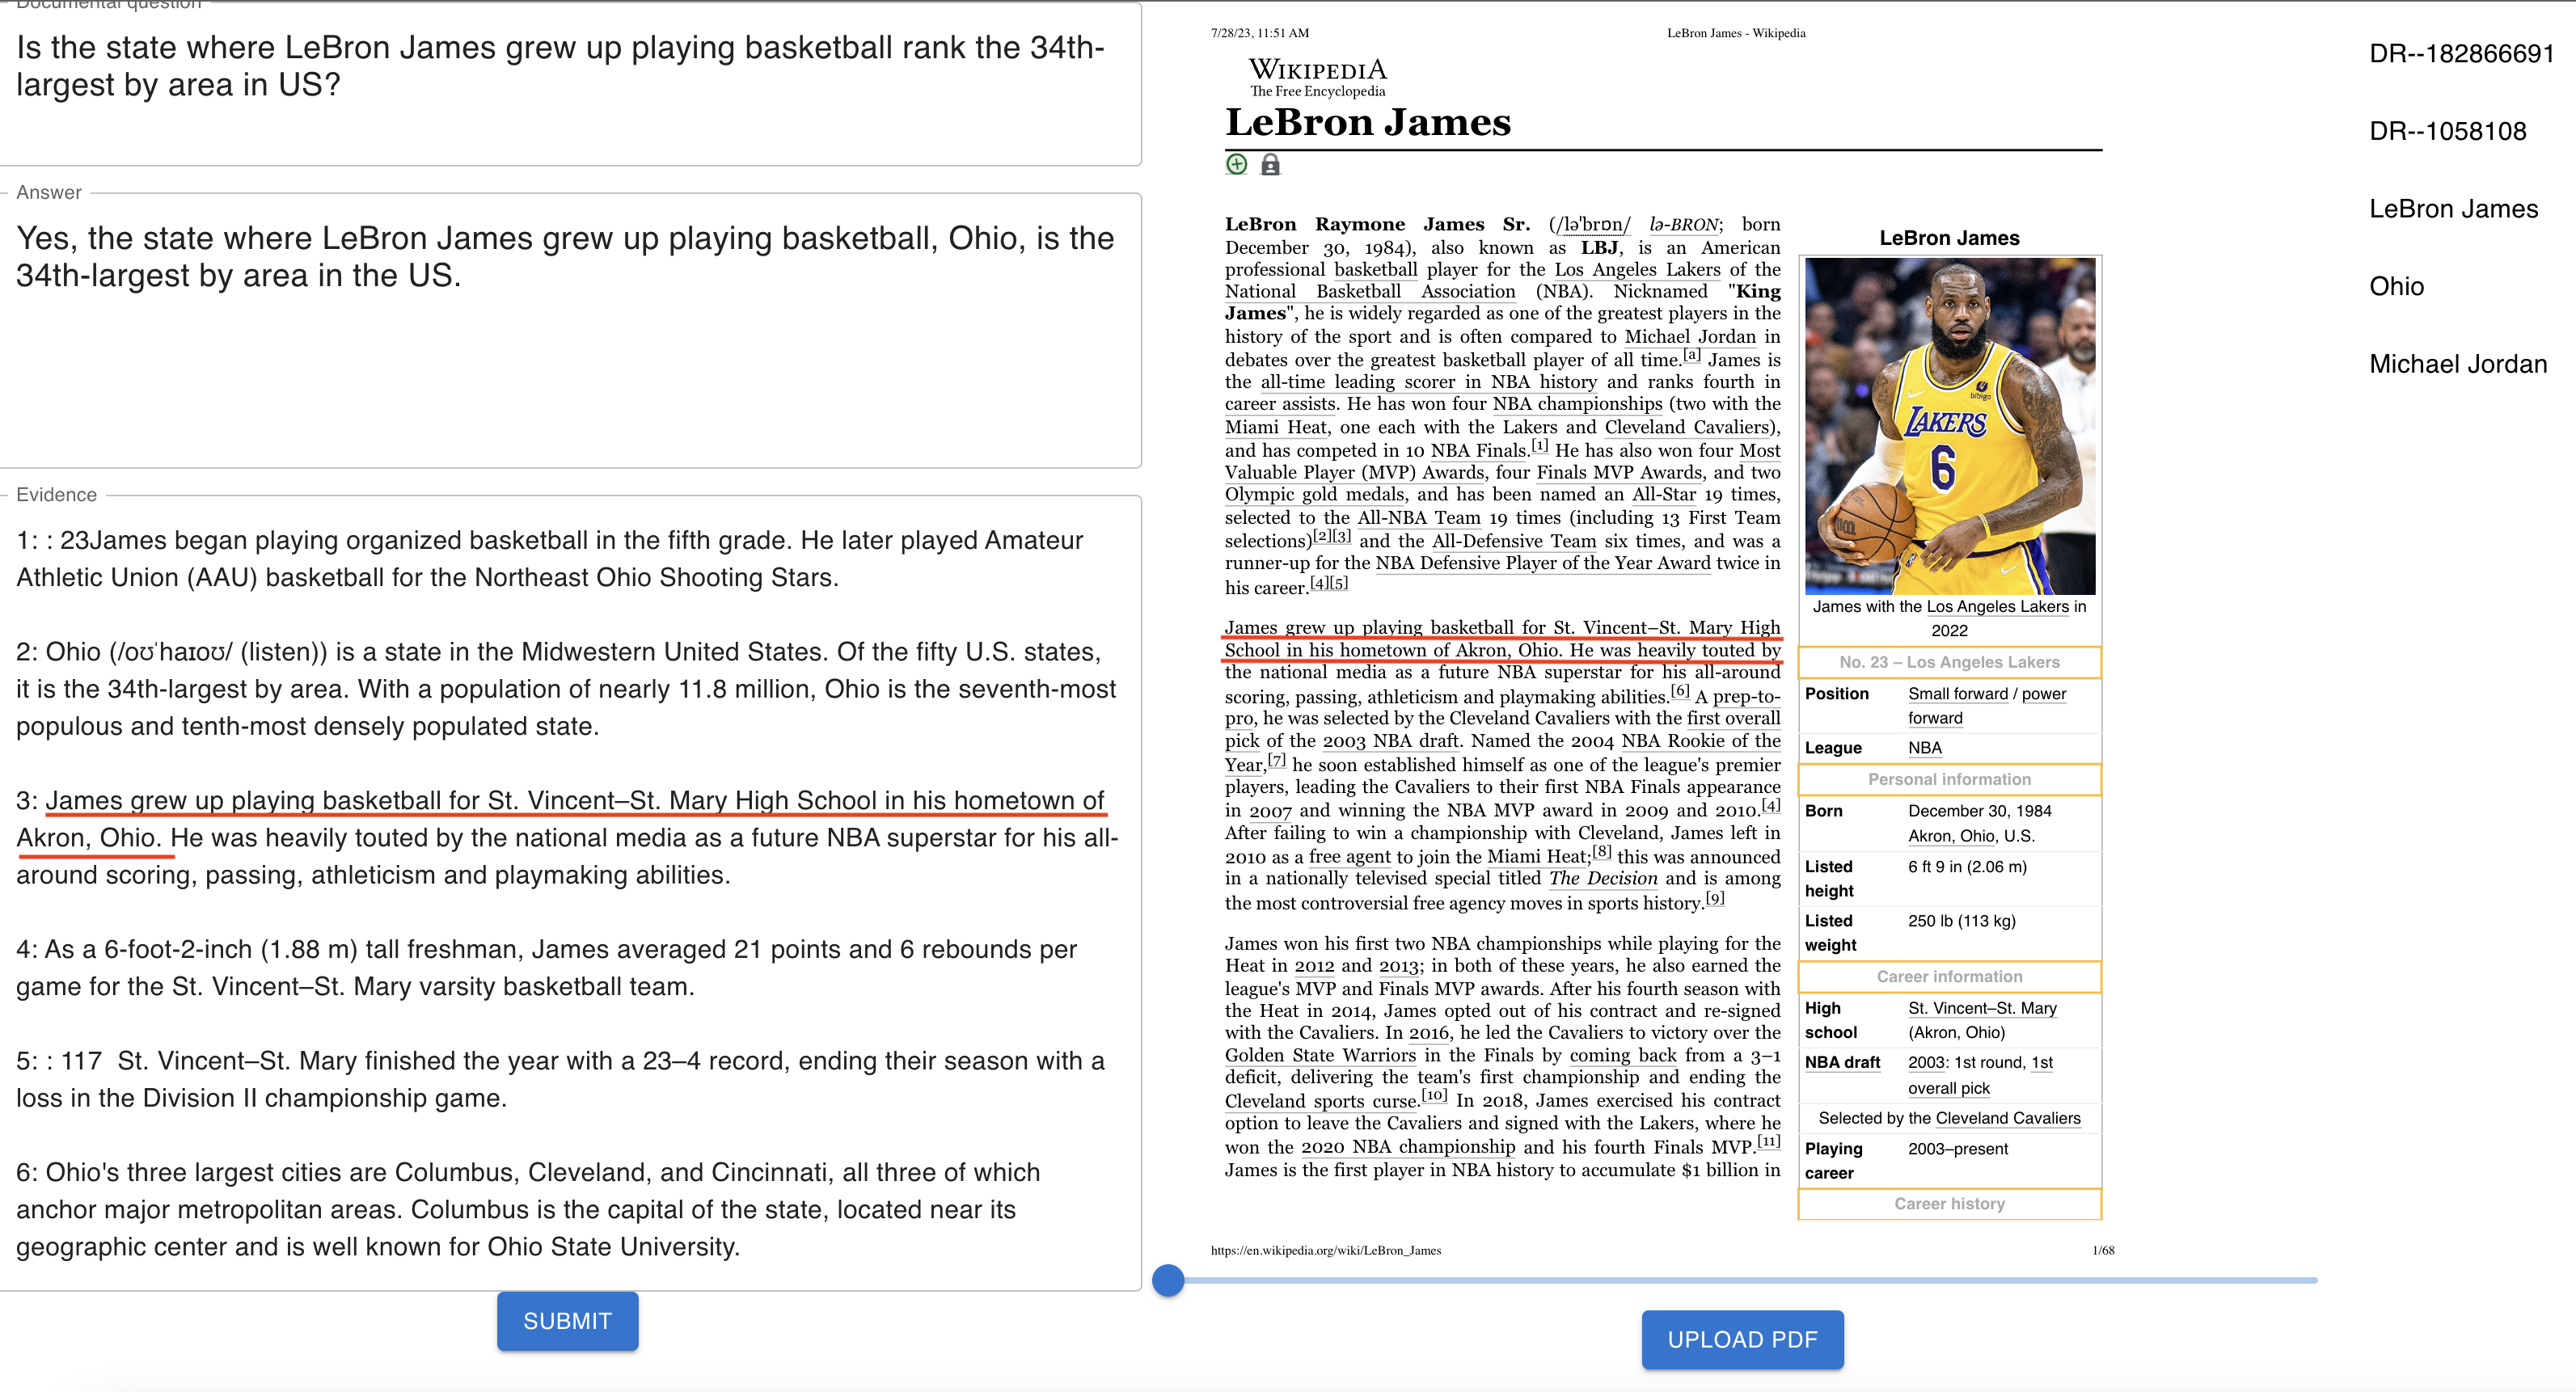
\includegraphics[width=\textwidth]{Figure/LBJOhio-ex1.png}
    \caption{Multi-document Bridging Question asking the information about Lebron James and State Ohio. It requires to first retrieve the sentence stating the state where Lebron James grew up playing basketball.}
    \label{fig-LBJOhio-ex1}
\end{figure}

\begin{figure}[htbp!]
    \centering
    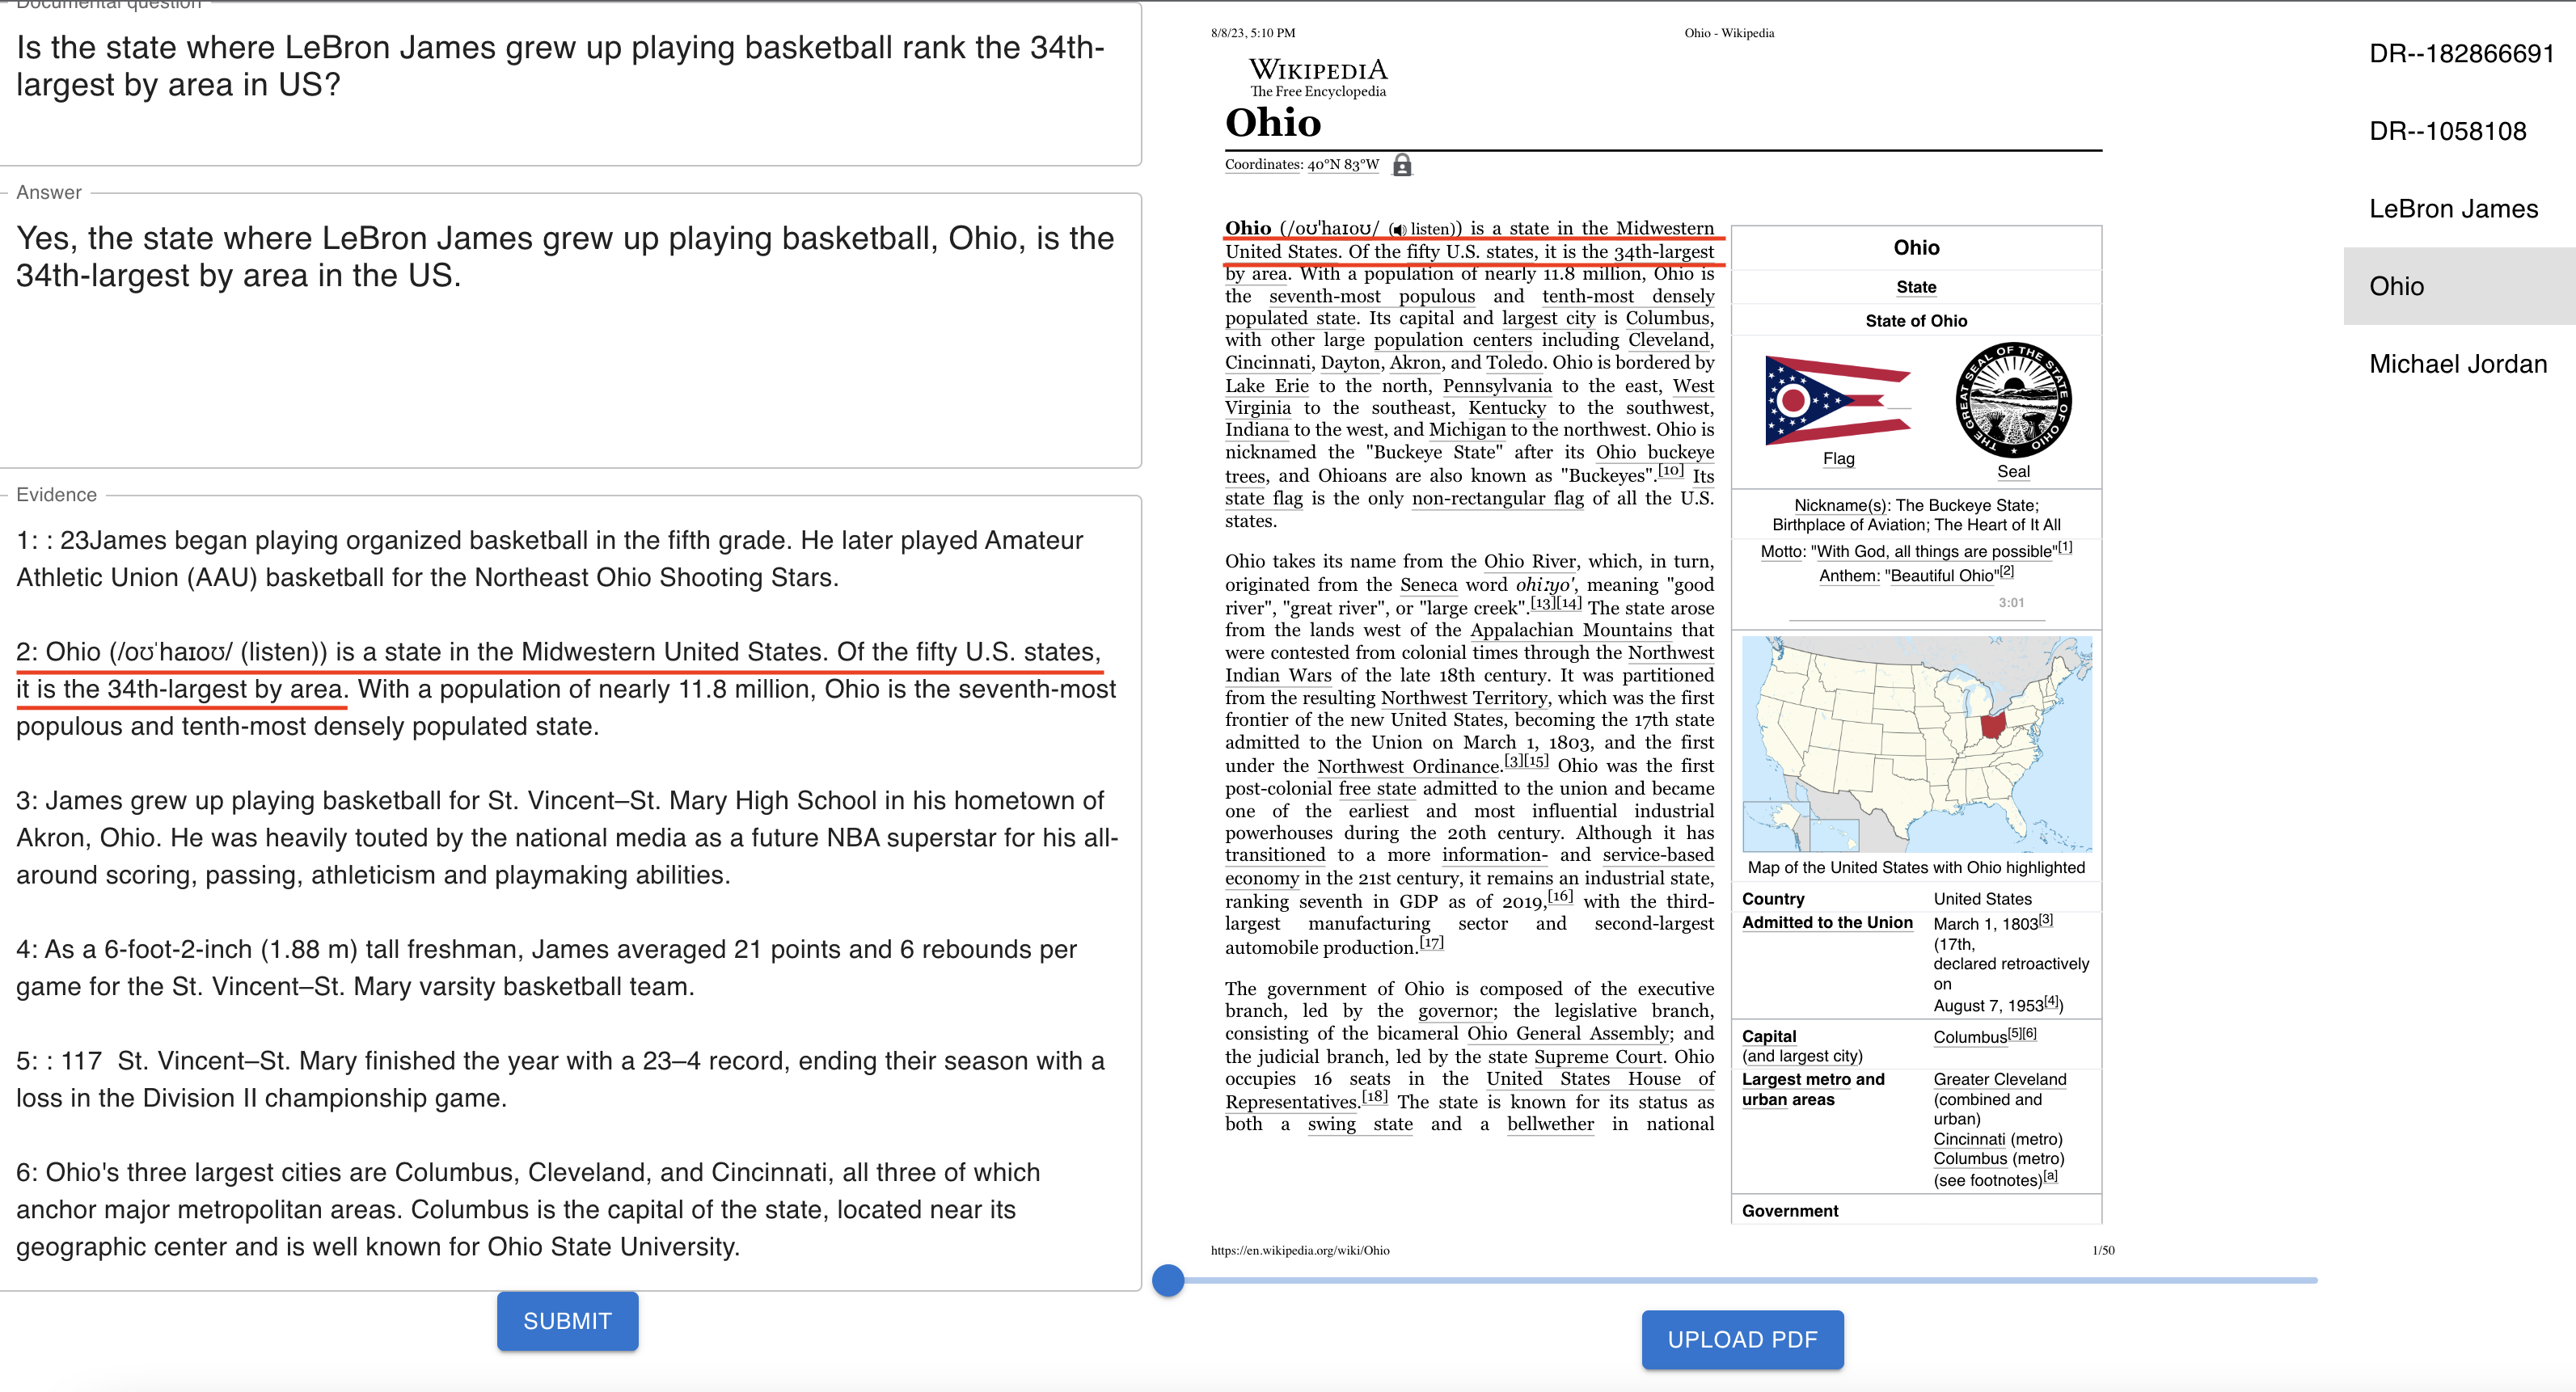
\includegraphics[width=\textwidth]{Figure/LBJOhio-ex2.png}
    \caption{Multi-document Bridging Question asking the information about Lebron James and State Ohio. Then it requires to judge whether the State Ohio ranks the 34th-largest by area in the US.}
    \label{fig-LBJOhio-ex2}
\end{figure}

\begin{figure}[htbp!]
    \centering
    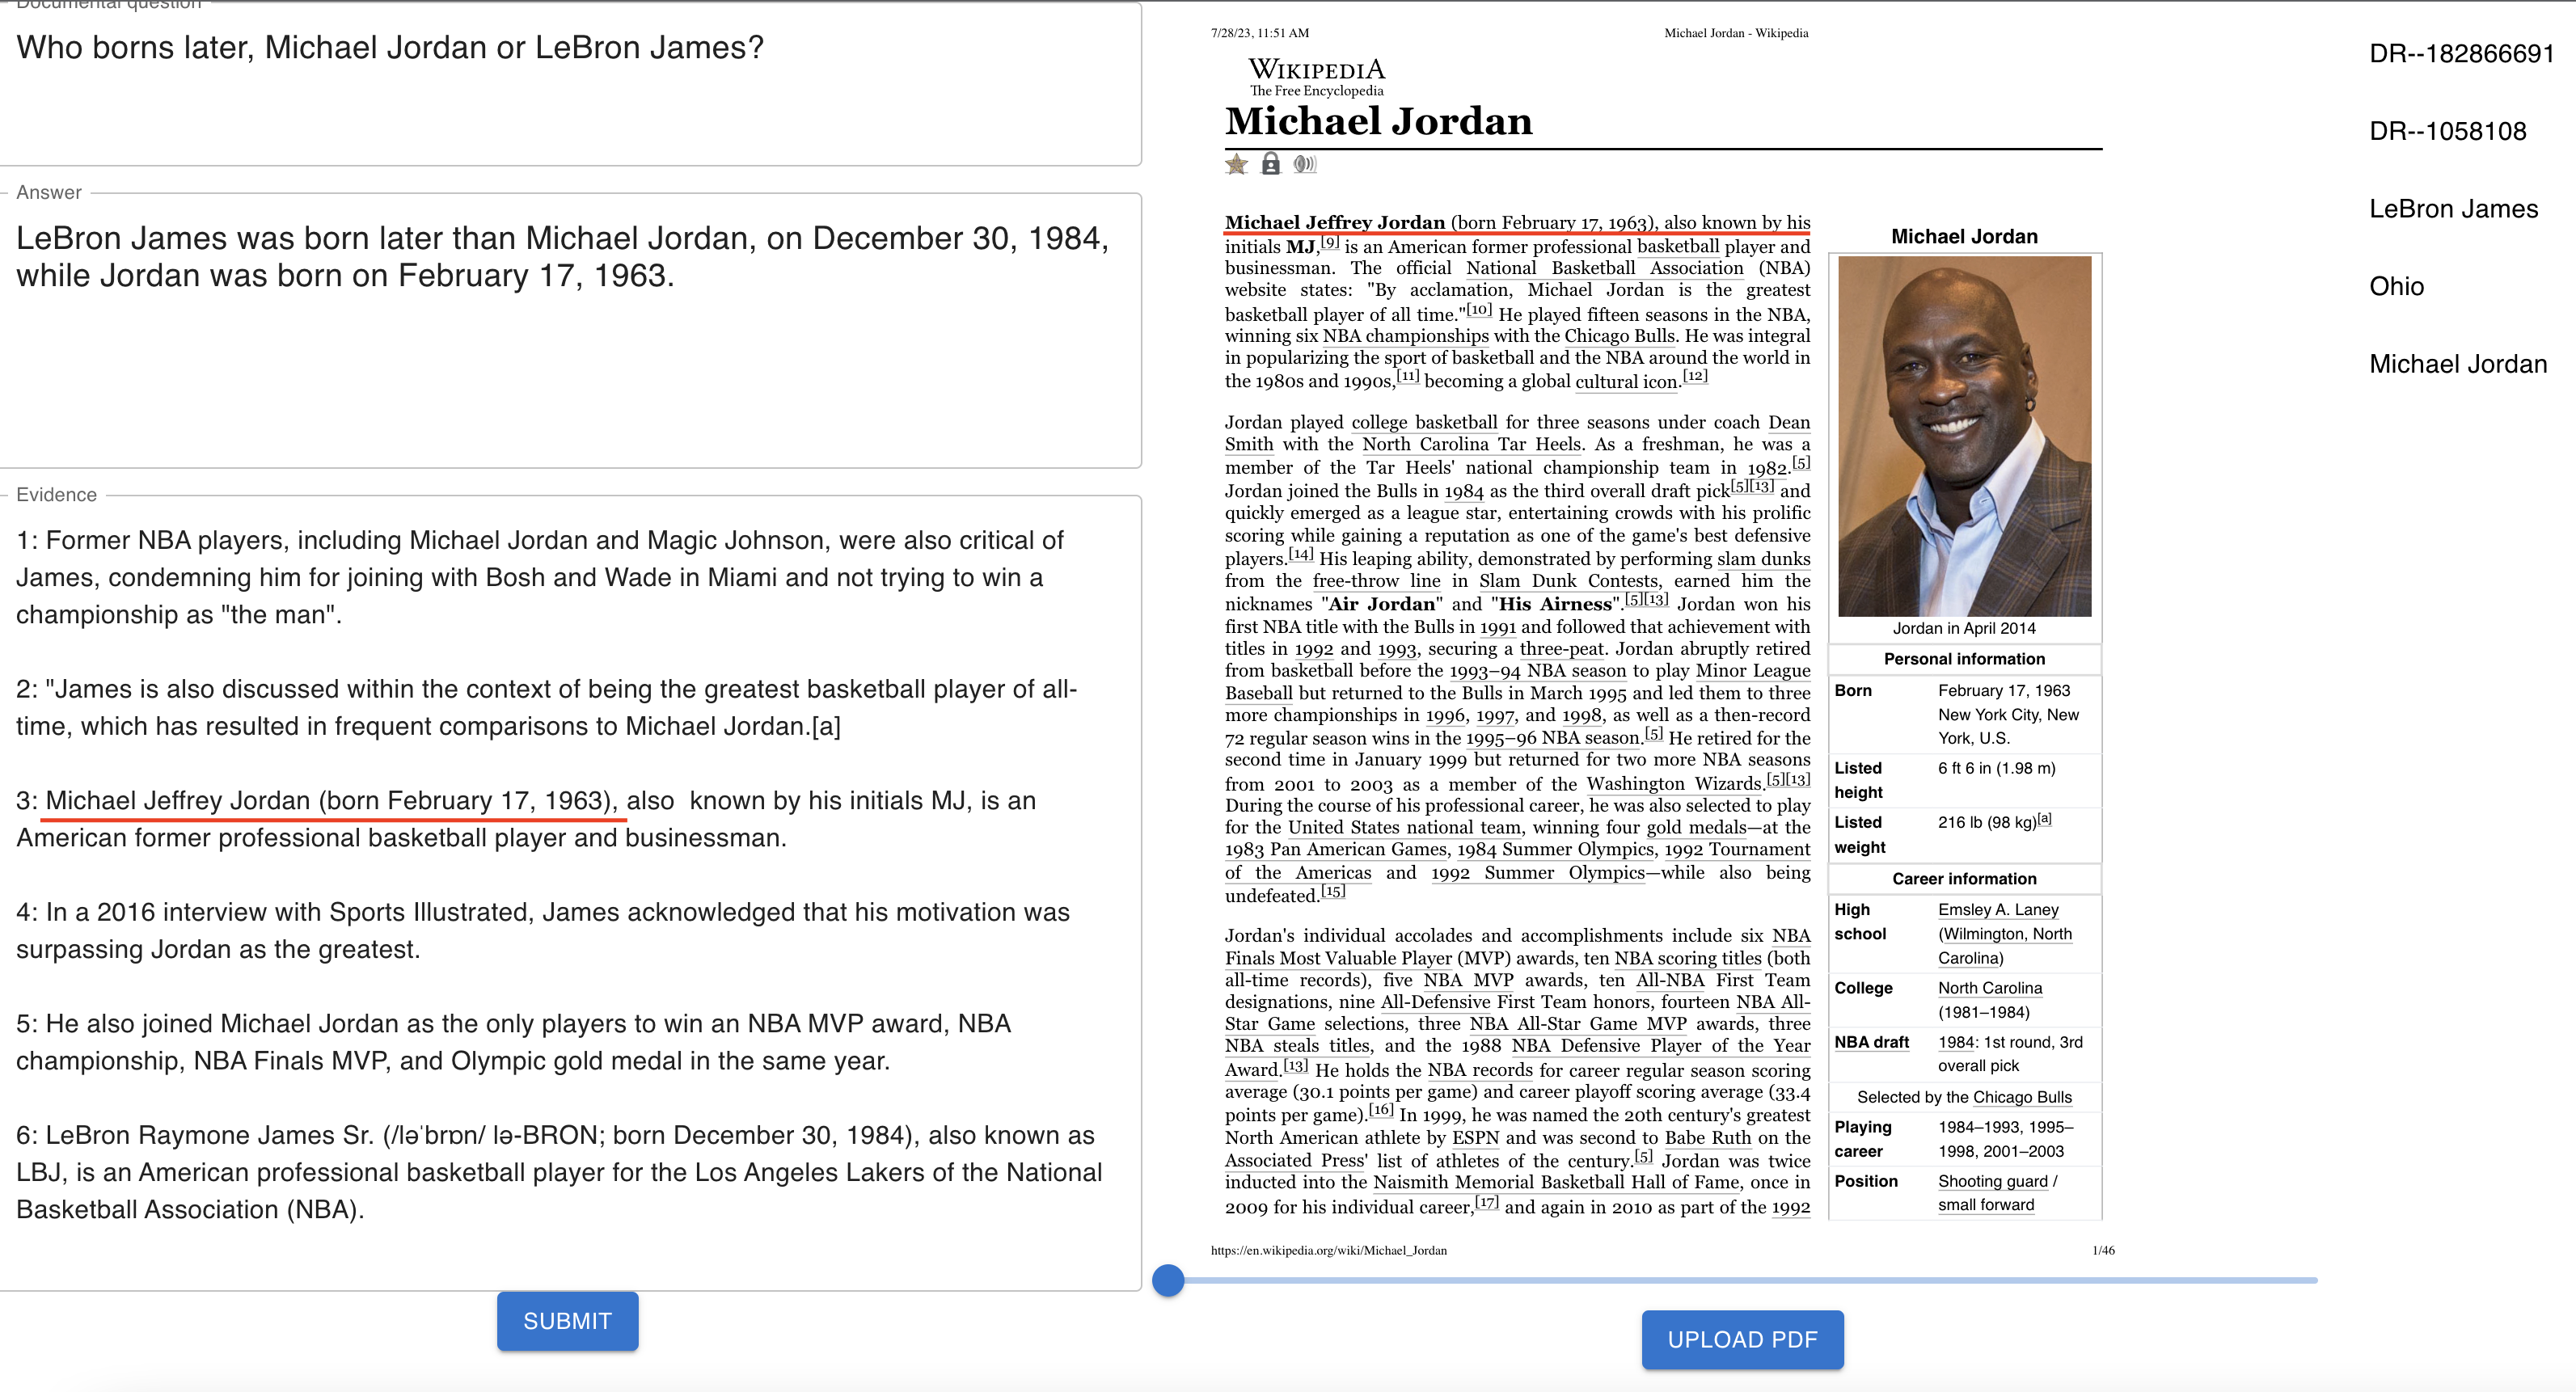
\includegraphics[width=\textwidth]{Figure/MJLBJ-ex.png}
    \caption{Multi-document Comparing Question comparing Lebron James and Michael Jordan. It requires the birthday information of Lebron and Jordan.}
    \label{fig-MJLBJ-ex1}
\end{figure}

\begin{figure}[htbp!]
    \centering
    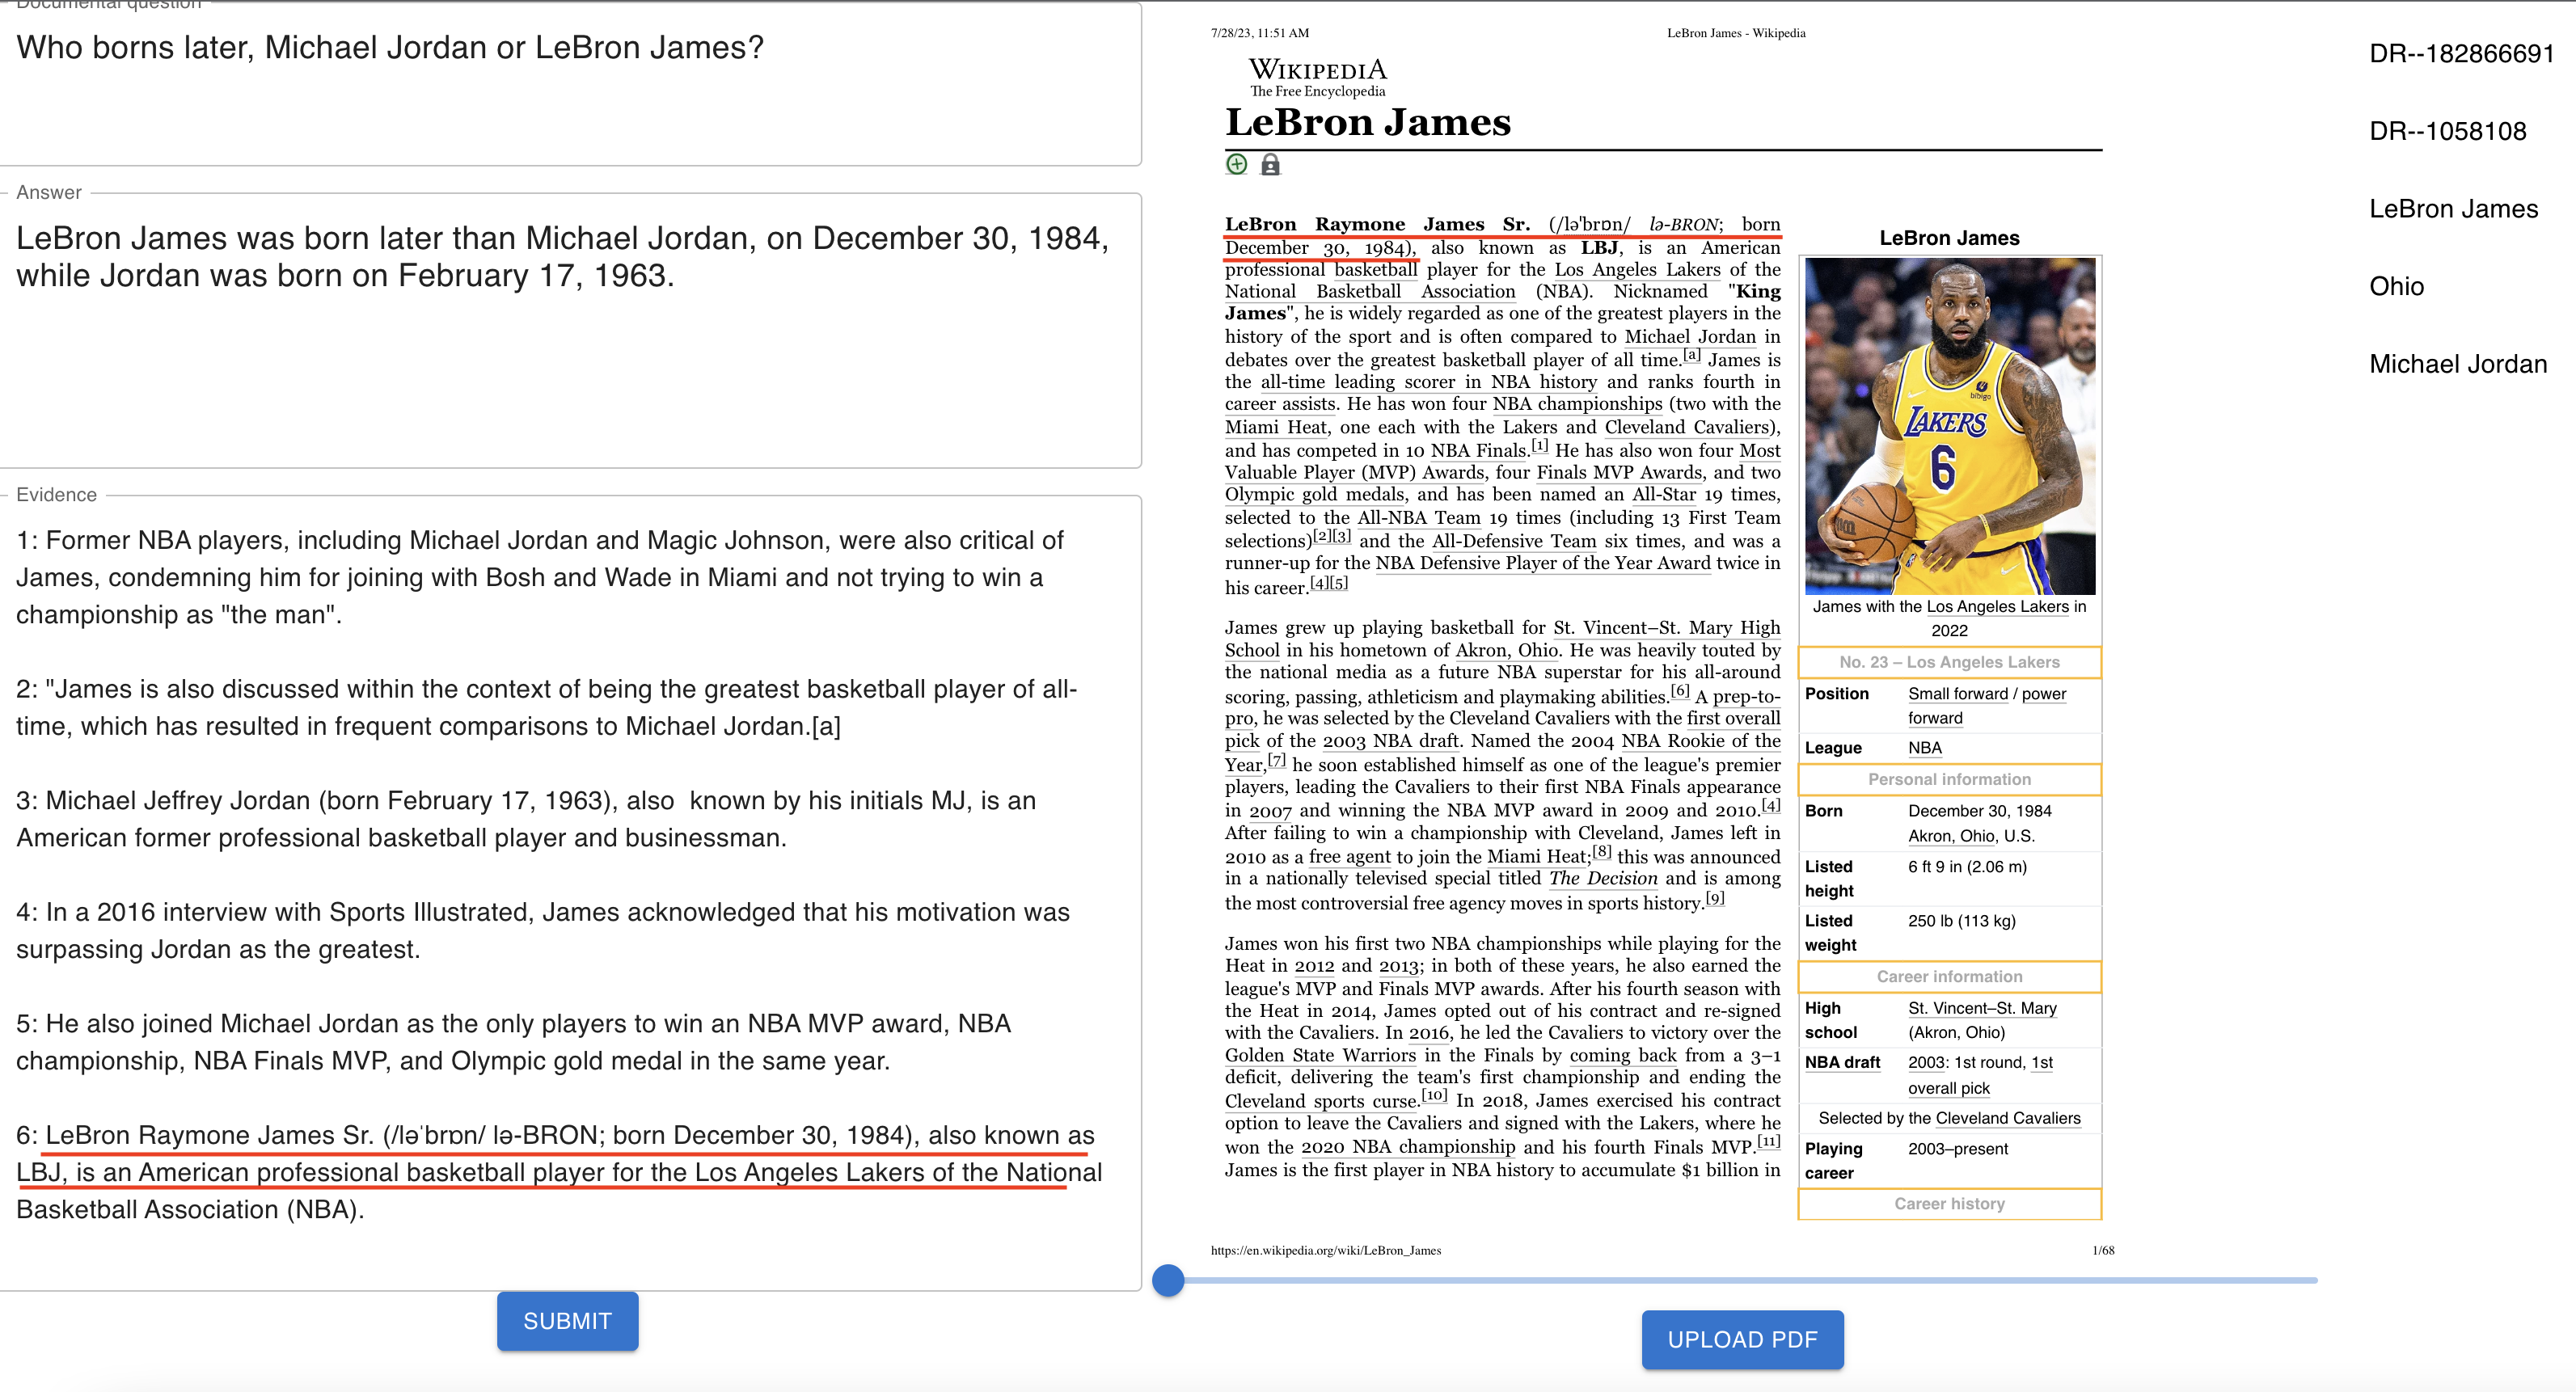
\includegraphics[width=\textwidth]{Figure/MJLBJ-ex2.png}
    \caption{Multi-document Comparing Question comparing Lebron James and Michael Jordan.  It requires the birthday information of Lebron and Jordan.}
    \label{fig-MJLBJ-ex2}
\end{figure}

\newpage
\subsection{Visualizing the Reasoning-and-Retrieving Process of LM-guided Graph Traverser}\label{sec-visualreason}

\begin{figure}[htbp!]
    \centering
    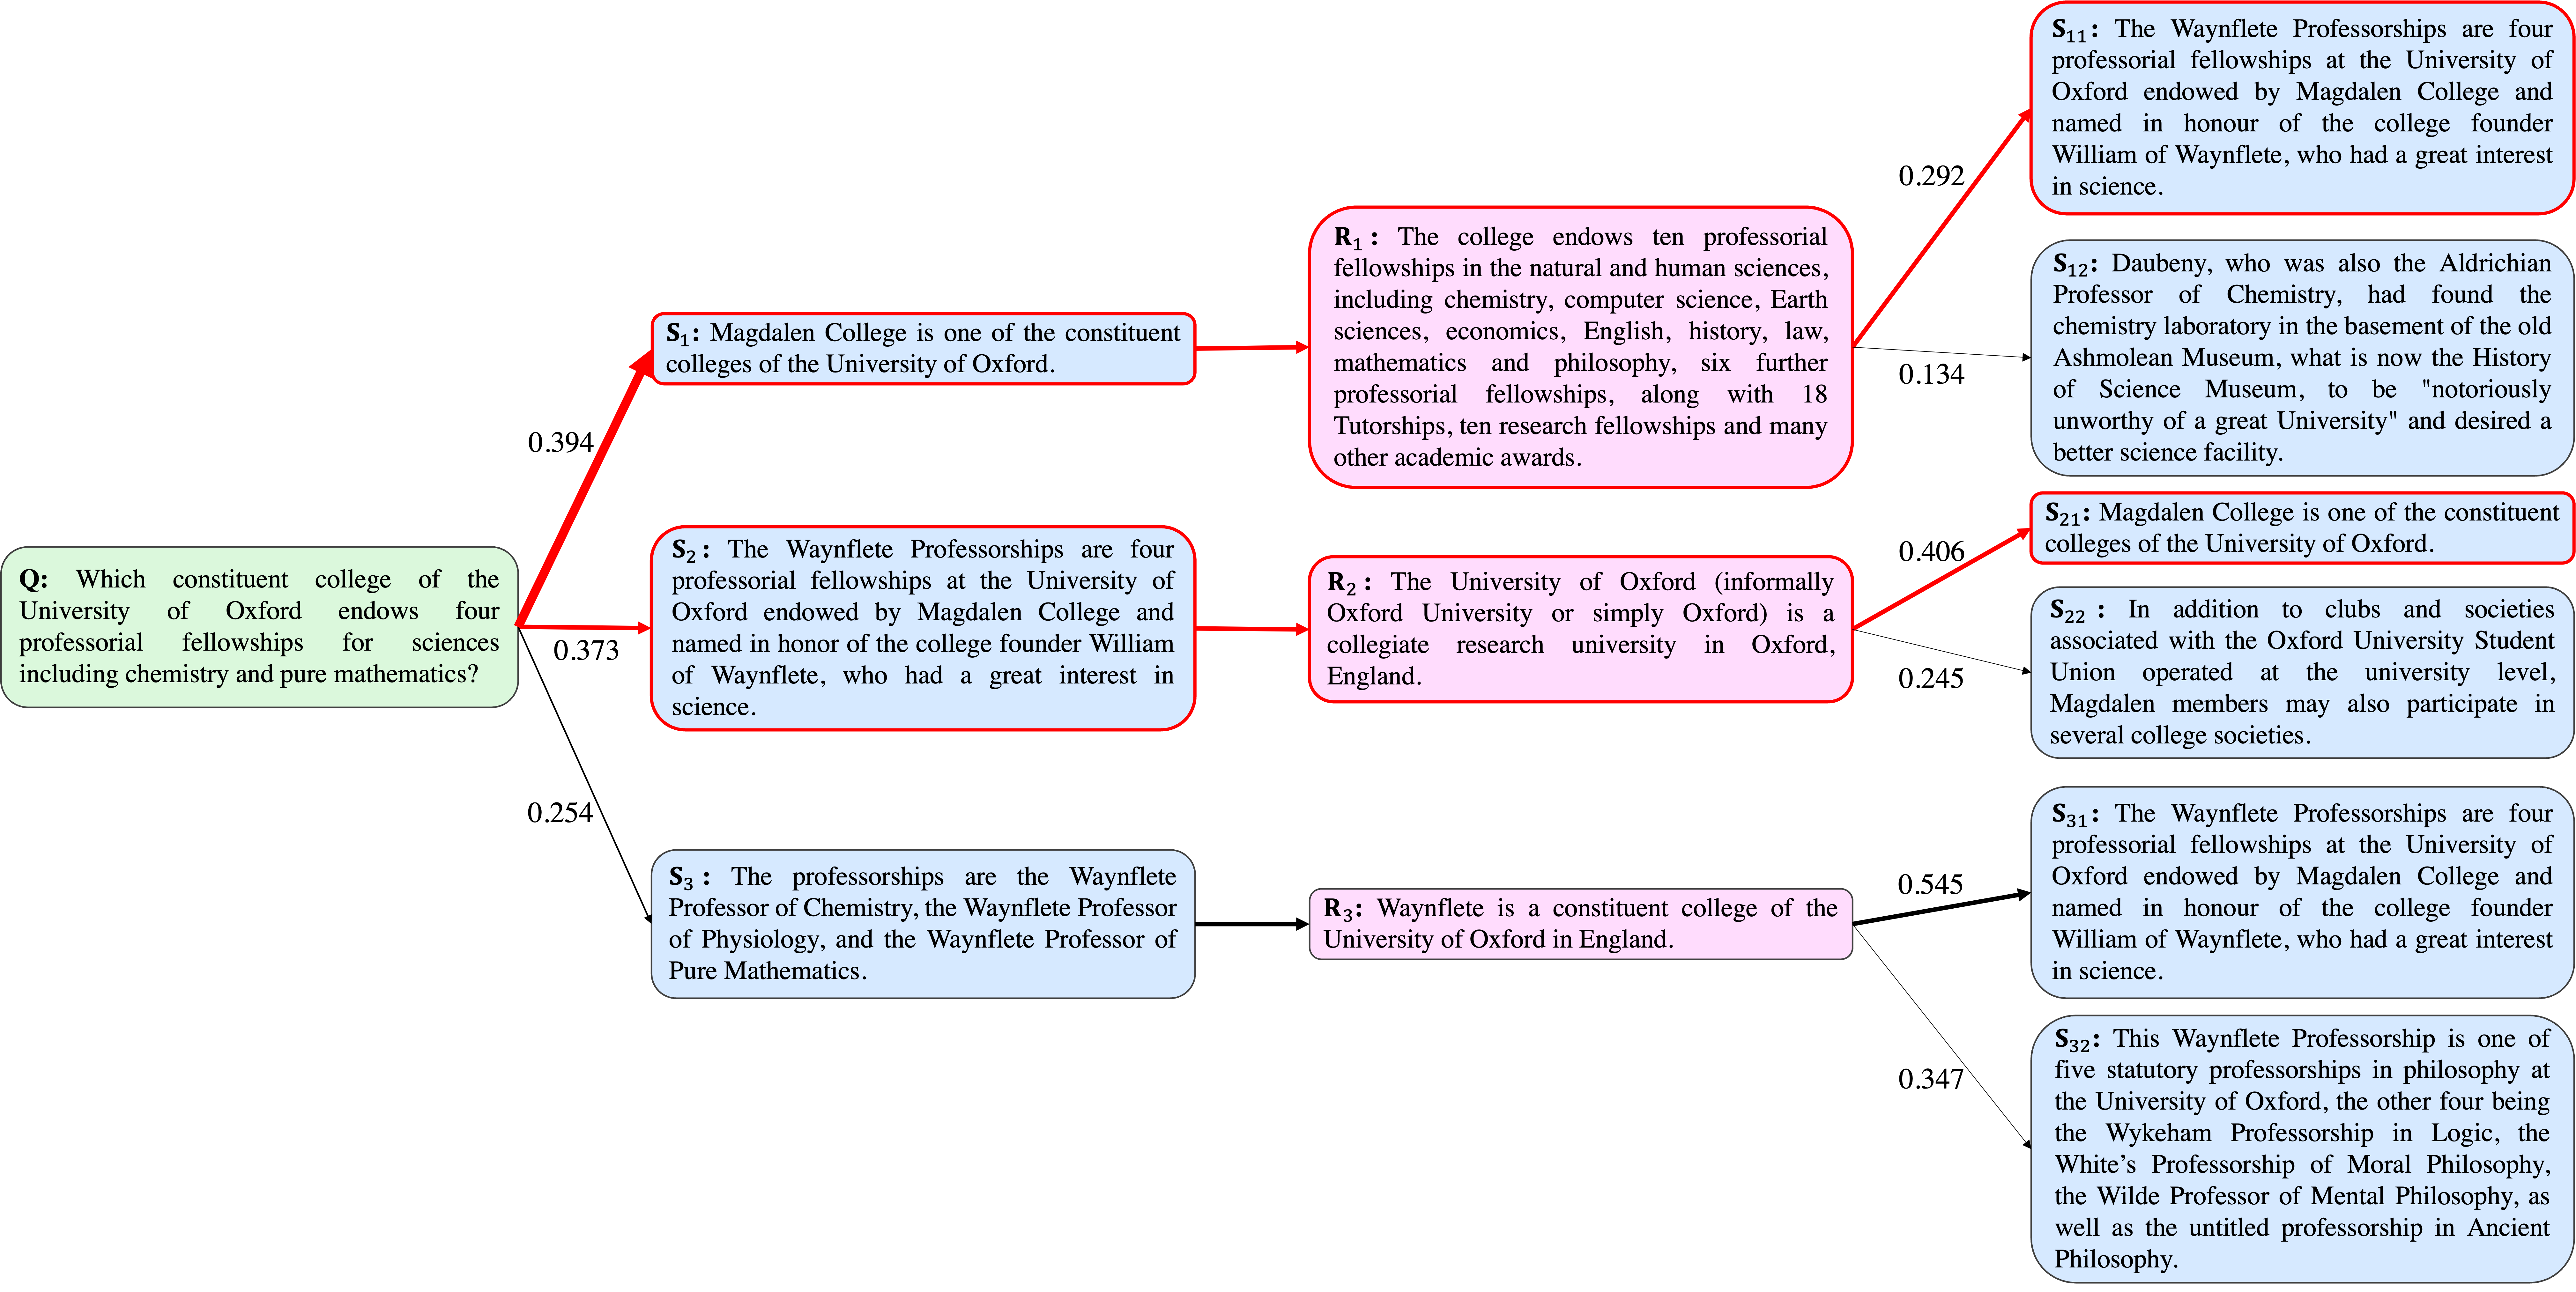
\includegraphics[width=\textwidth]{Figure/multi-hop_visual1.png}
    \caption{Visualizing the graph traversal over MD-QA-Example 1.}
    \label{fig-visual-ex1}
\end{figure}

\begin{figure}[htbp!]
    \centering
    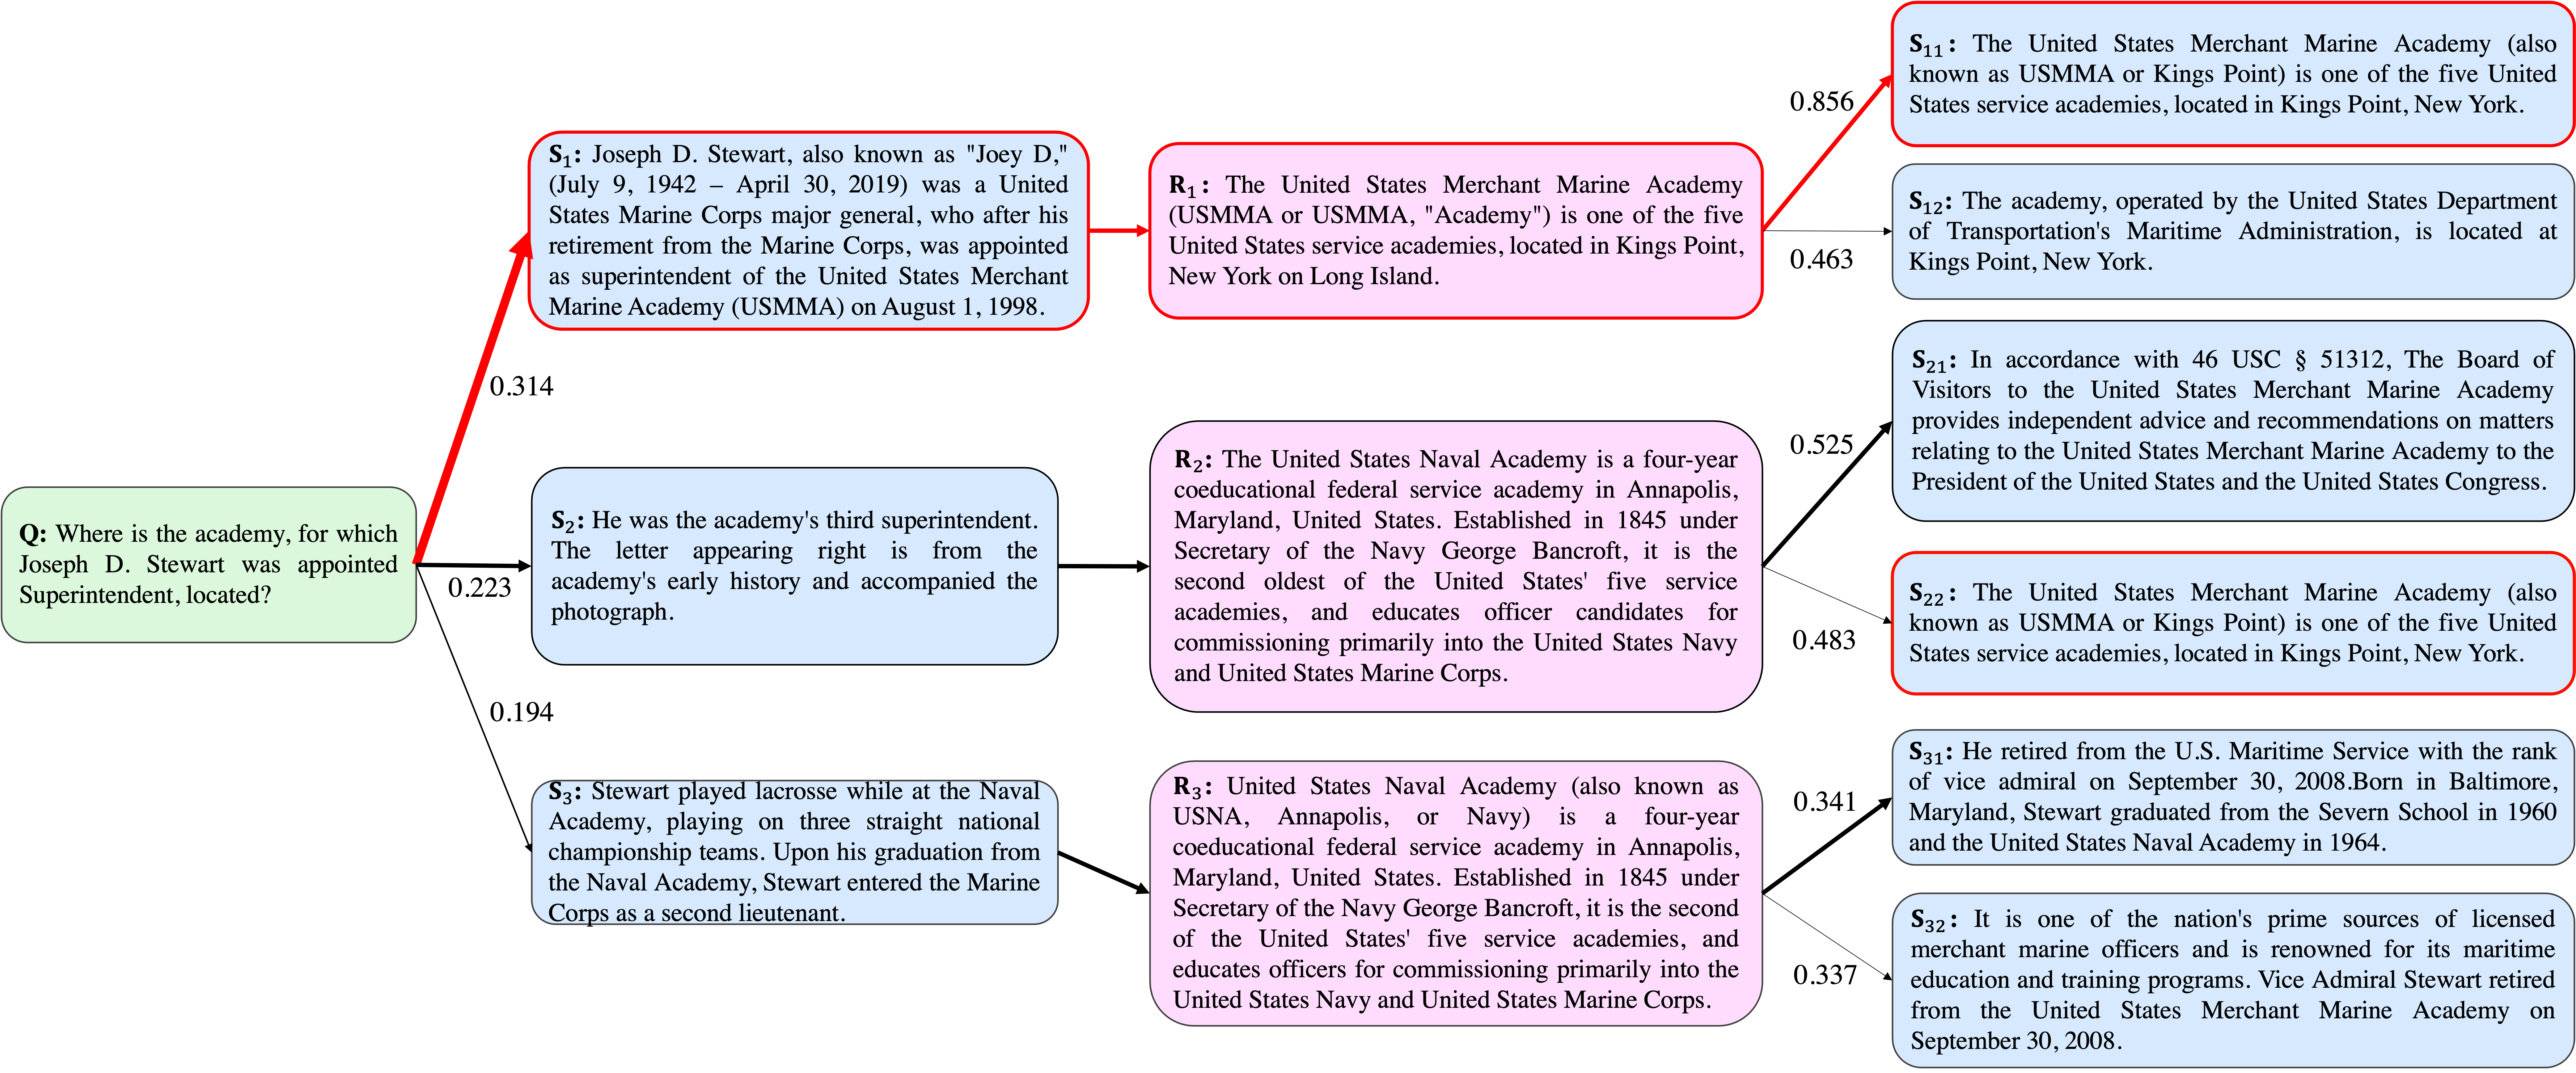
\includegraphics[width=\textwidth]{Figure/multi-hop_visual2.png}
    \caption{Visualizing the graph traversal over MD-QA-Example 2.}
    \label{fig-visual-ex2}
\end{figure}

\newpage
\subsection{Prompt template used throughout this work}\label{sec-prompt}
\colorlet{shadecolor}{gray!10}
\UseRawInputEncoding
\lstset{breaklines=true, columns=fullflexible, backgroundcolor=\color{shadecolor}}
\lstinputlisting[basicstyle=\footnotesize, title={Examples of the Instruction Data for Fine-tuning LLaMA and T5-Large.}, caption={Examples of the Instruction Data for Fine-tuning LLaMA.}, label={list-InstructData}]{prompts/hotpotqa_instruction.txt}


\colorlet{shadecolor}{gray!10}
\UseRawInputEncoding
\lstset{breaklines=true, columns=fullflexible, backgroundcolor=\color{shadecolor}}
\lstinputlisting[basicstyle=\footnotesize, title={Example of the Prompt for QA without Retrieved Contexts.}, caption={Example of the Prompt for QA without Retrieved Contexts.}, label={list-Prompt1}]{prompts/qa.txt}


\colorlet{shadecolor}{gray!10}
\UseRawInputEncoding
\lstset{breaklines=true, columns=fullflexible, backgroundcolor=\color{shadecolor}}
\lstinputlisting[basicstyle=\footnotesize, title={Example of the Prompt for QA with Retrieved Contexts.}, caption={Example of the Prompt for QA with Retrieved Contexts.}, label={list-Prompt2}]{prompts/qac.txt}

\newpage
\colorlet{shadecolor}{gray!10}
\UseRawInputEncoding
\lstset{breaklines=true, columns=fullflexible, backgroundcolor=\color{shadecolor}}
\lstinputlisting[basicstyle=\footnotesize, title={Example of the Prompt for QA with Retrieved Contexts for MDR, KGP-T5, KGP-LLaMA and KGP-MDR.}, caption={Example of the Prompt for QA with Retrieved Contexts for MDR, KGP-T5, KGP-LLaMA and KGP-MDR.}, label={list-Prompt3}]{prompts/qac_mdr.txt}


\colorlet{shadecolor}{gray!10}
\UseRawInputEncoding
\lstset{breaklines=true, columns=fullflexible, backgroundcolor=\color{shadecolor}}
\lstinputlisting[basicstyle=\footnotesize, title={Example of the Prompt for Grading QA.}, caption={Example of the Prompt for Grading QA.}, label={list-Prompt4}]{prompts/qa_grade.txt}





